%%%%%%%%%%%%%%%%%%%%%%%%%%%%%%%%%%%%%%%%%%%%%%%%%%%
%
%  New template code for TAMU Theses and Dissertations starting Fall 2012.  
%  For more info about this template or the 
%  TAMU LaTeX User's Group, see http://www.howdy.me/.
%
%  Author: Wendy Lynn Turner 
%	 Version 1.0 
%  Last updated 8/5/2012
%
%%%%%%%%%%%%%%%%%%%%%%%%%%%%%%%%%%%%%%%%%%%%%%%%%%%
%%%                           APPENDIX A
%%%%%%%%%%%%%%%%%%%%%%%%%%%%%%%%%%%%%%%%%%%%%%%%%%%

\phantomsection

\chapter{\uppercase{$S_N$}}
\label{sec::appendix_SN}


\begin{figure}
\label{fig::Legendre_Polynomials}
\centering
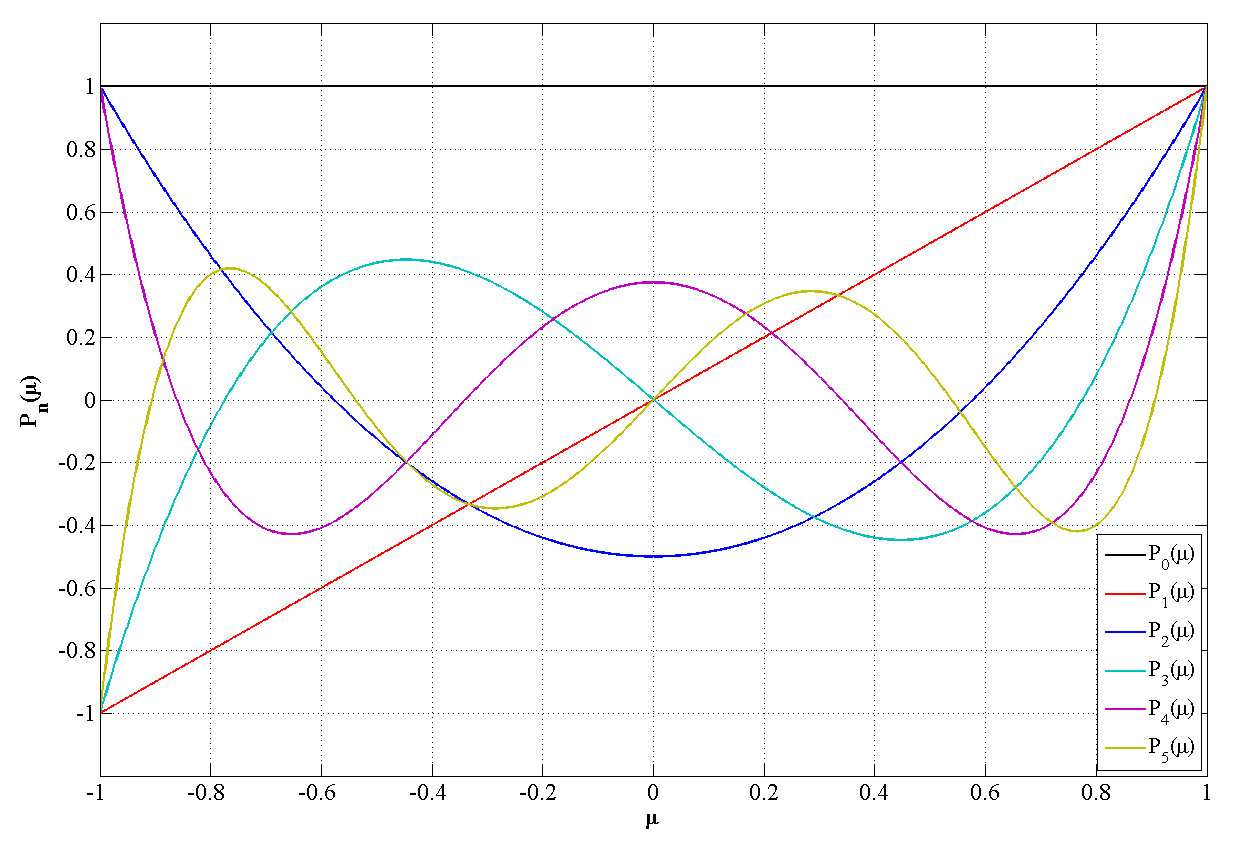
\includegraphics[width=\textwidth]{figures/appendices/legendre_polynomials.png}
\caption{Legendre polynomials of degrees 0 through 5.}
\end{figure}

% List of Spherical Harmonics Plots
\pagebreak

\begin{figure}
\label{fig::Sn_Y0}
\centering
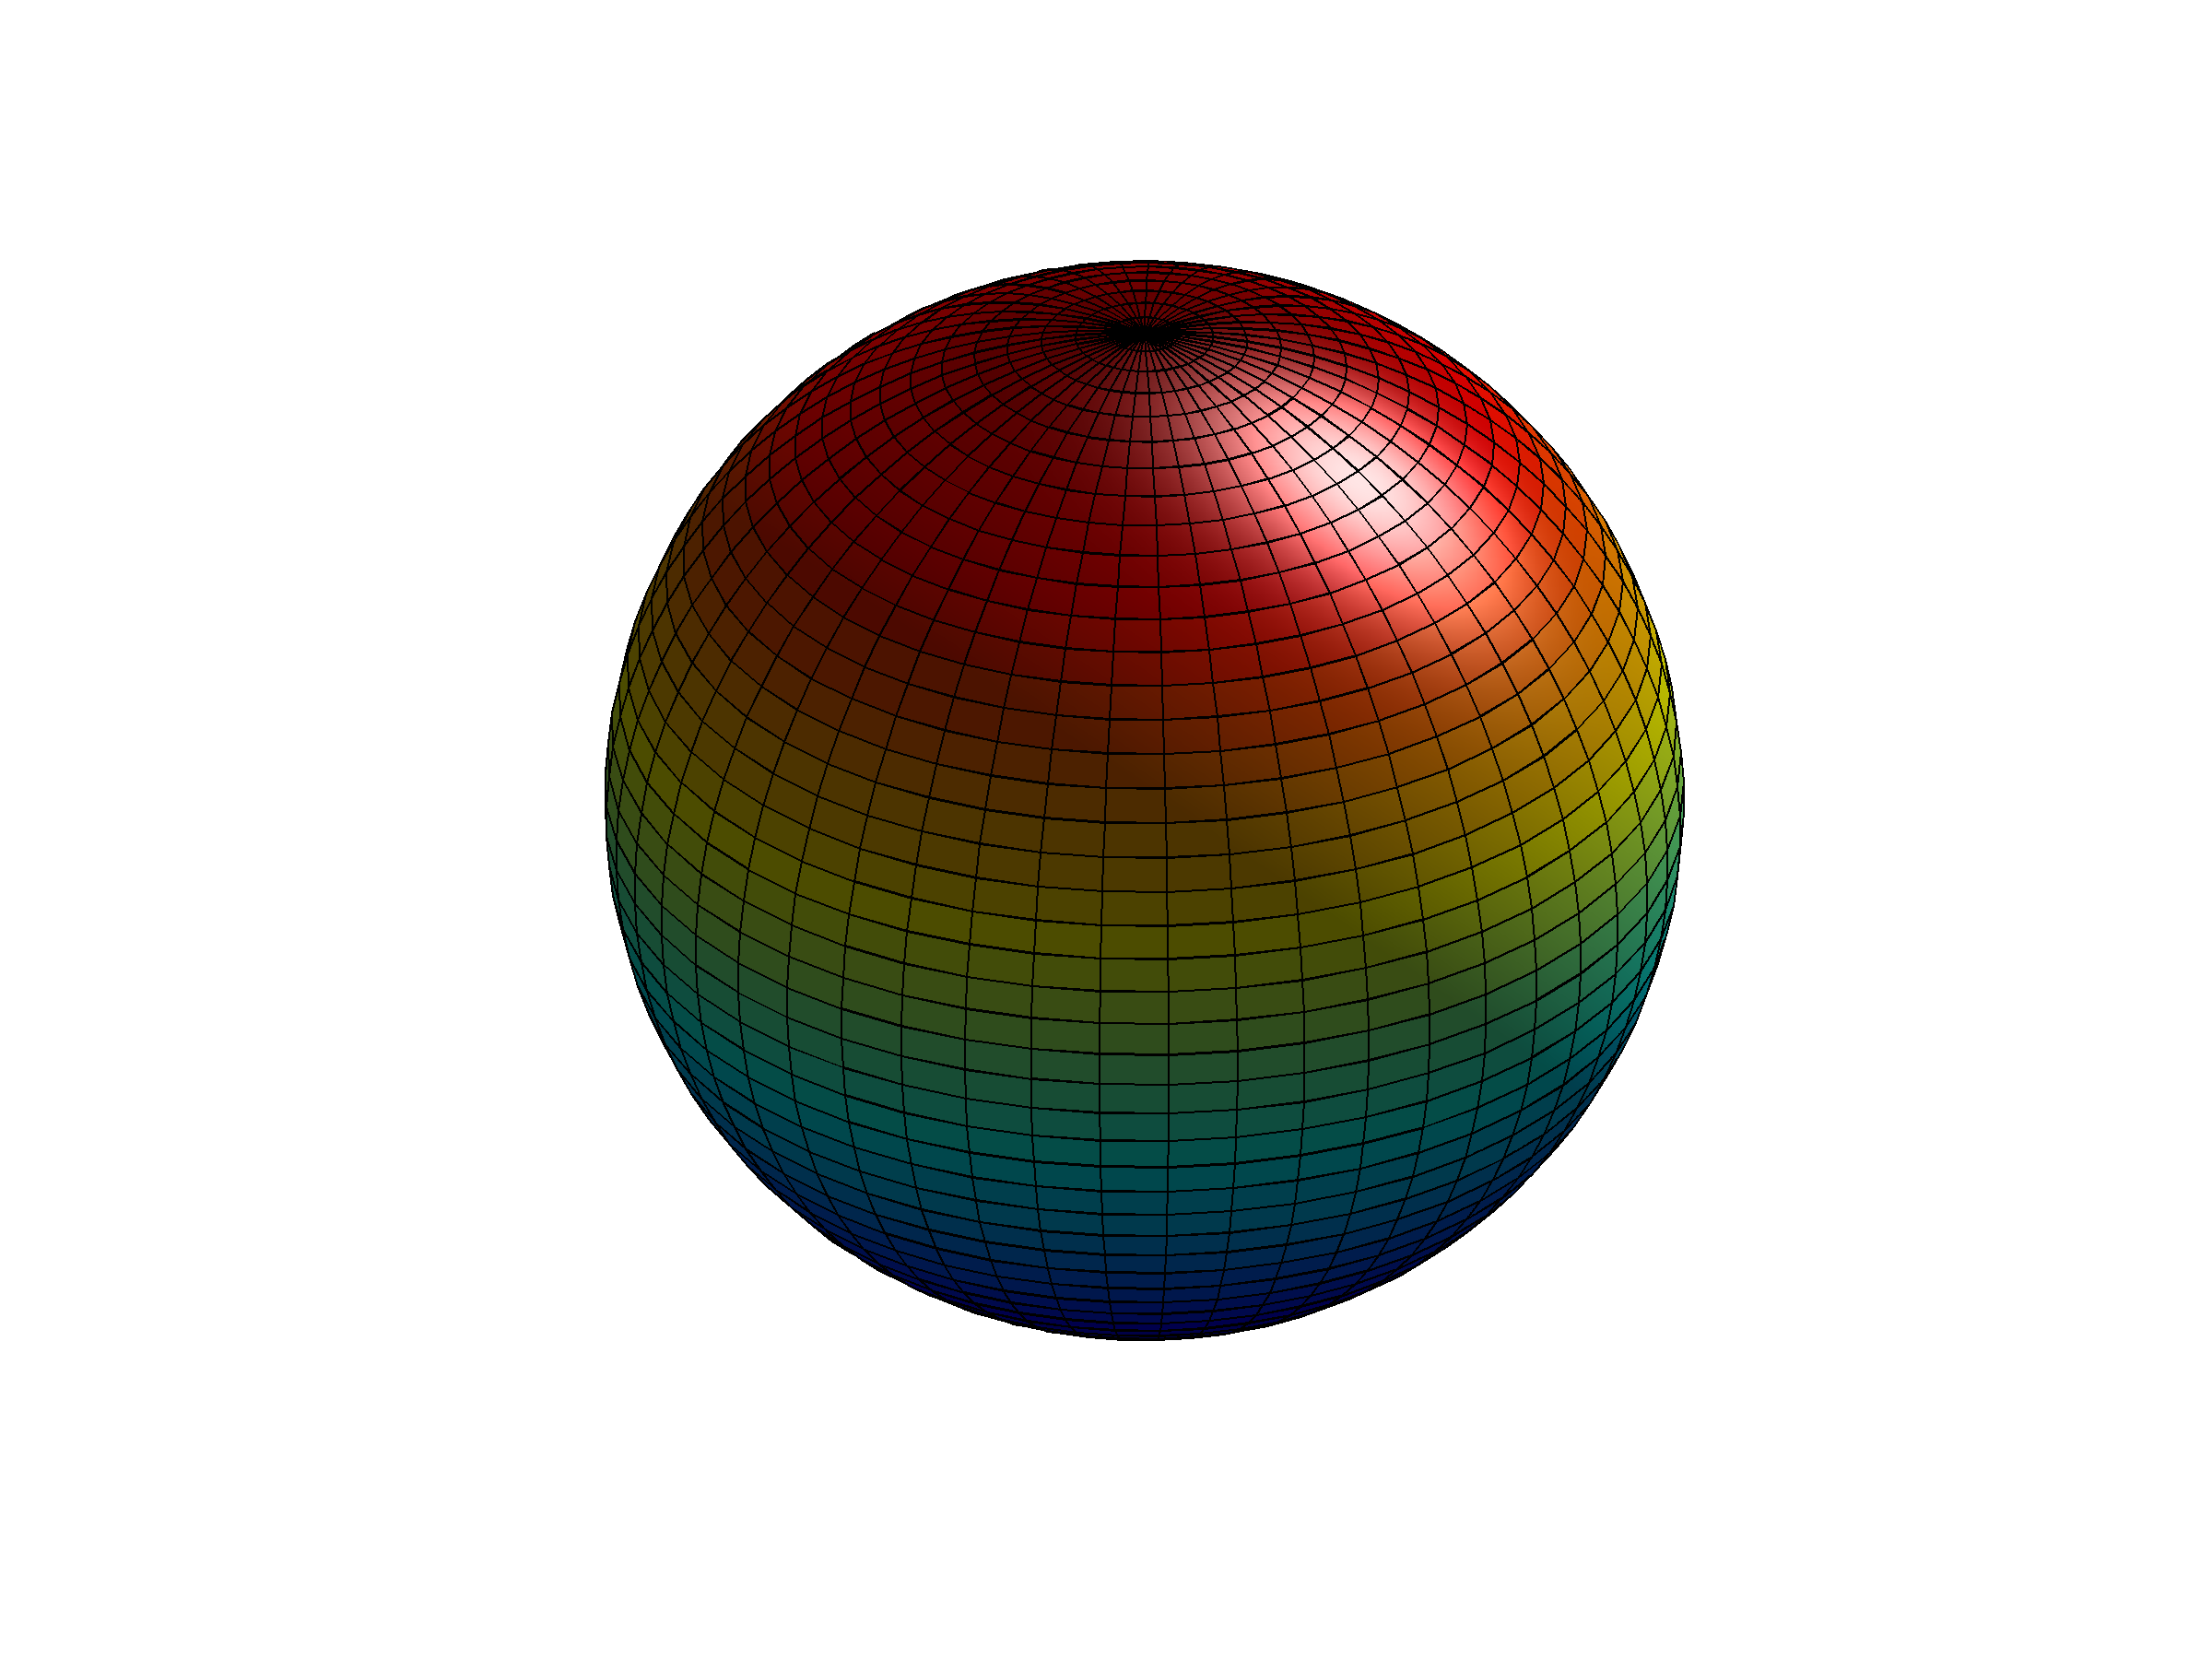
\includegraphics[width=0.45\textwidth]{figures/appendices/Y_0_0.png}
\caption{Spherical harmonic function of degree 0: $Y_{0}^{0}$.}
\end{figure}

\begin{figure}
\label{fig::Sn_Y1}
\centering
	\begin{subfigure}[b]{0.45\textwidth}
		\centering
		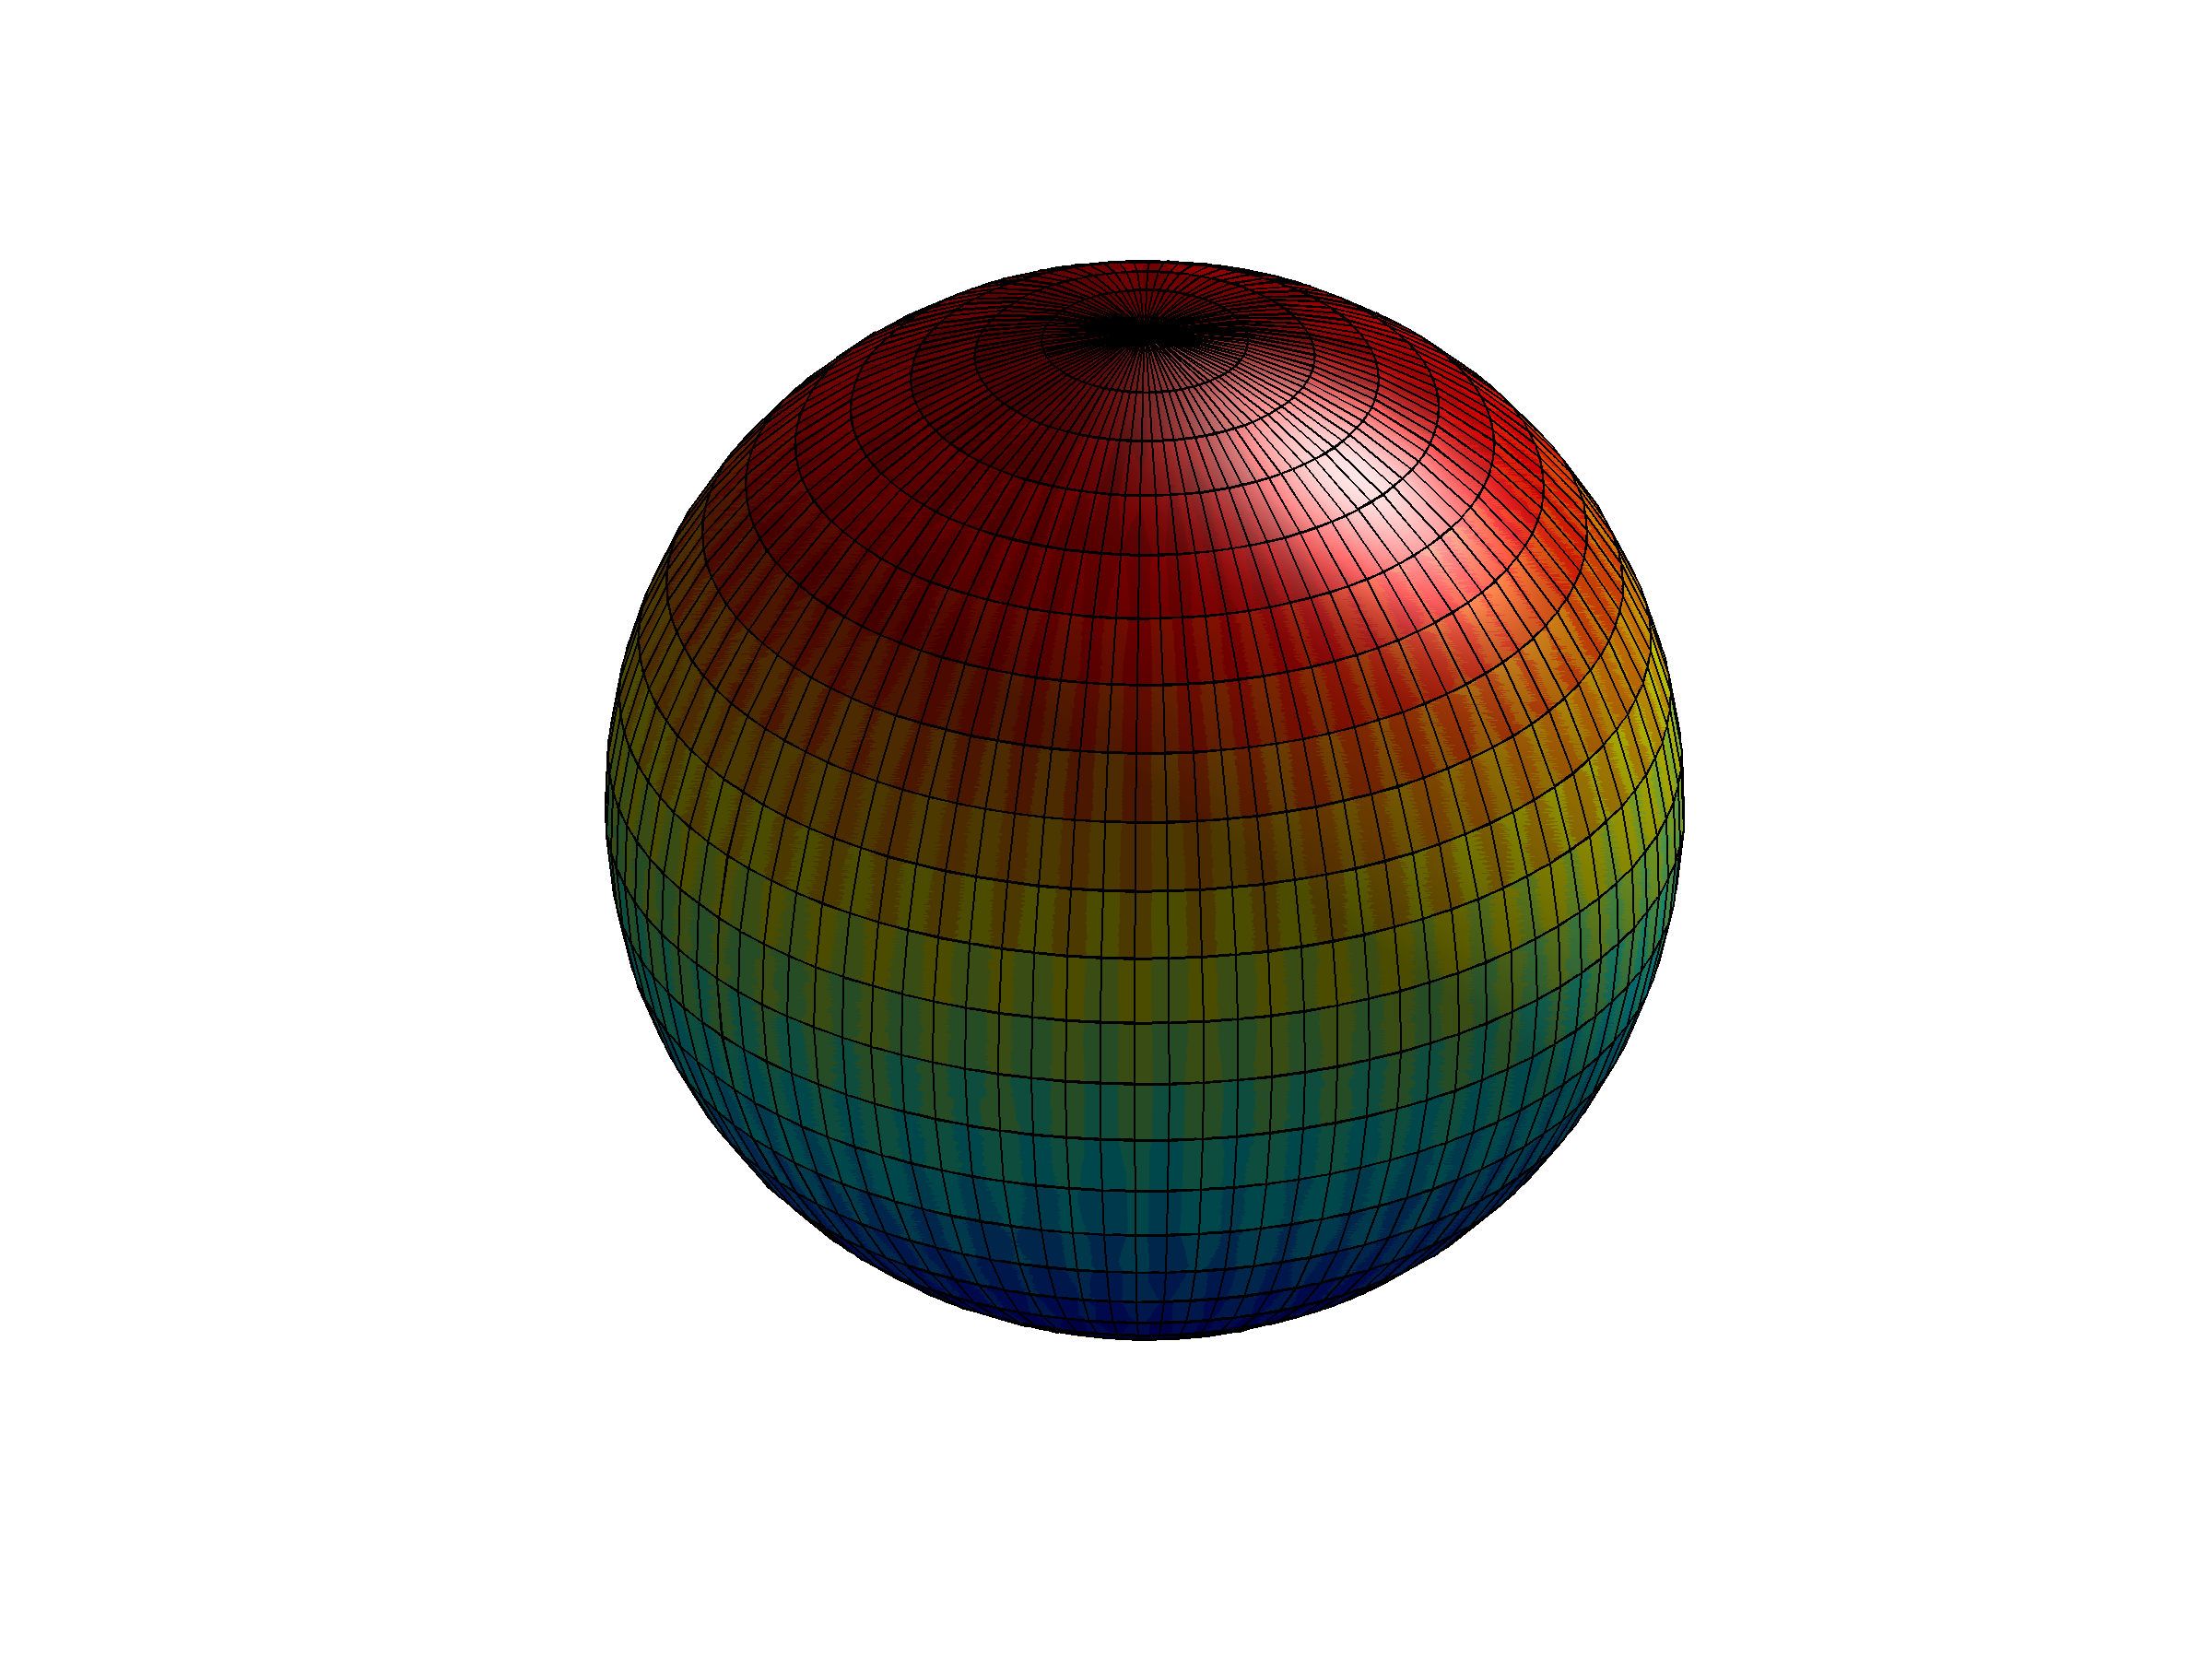
\includegraphics[width=\textwidth]{figures/appendices/Y_1_0.png}
		\caption{}
	\end{subfigure}
	\vfill
	\begin{subfigure}[b]{0.40\textwidth}
		\centering
		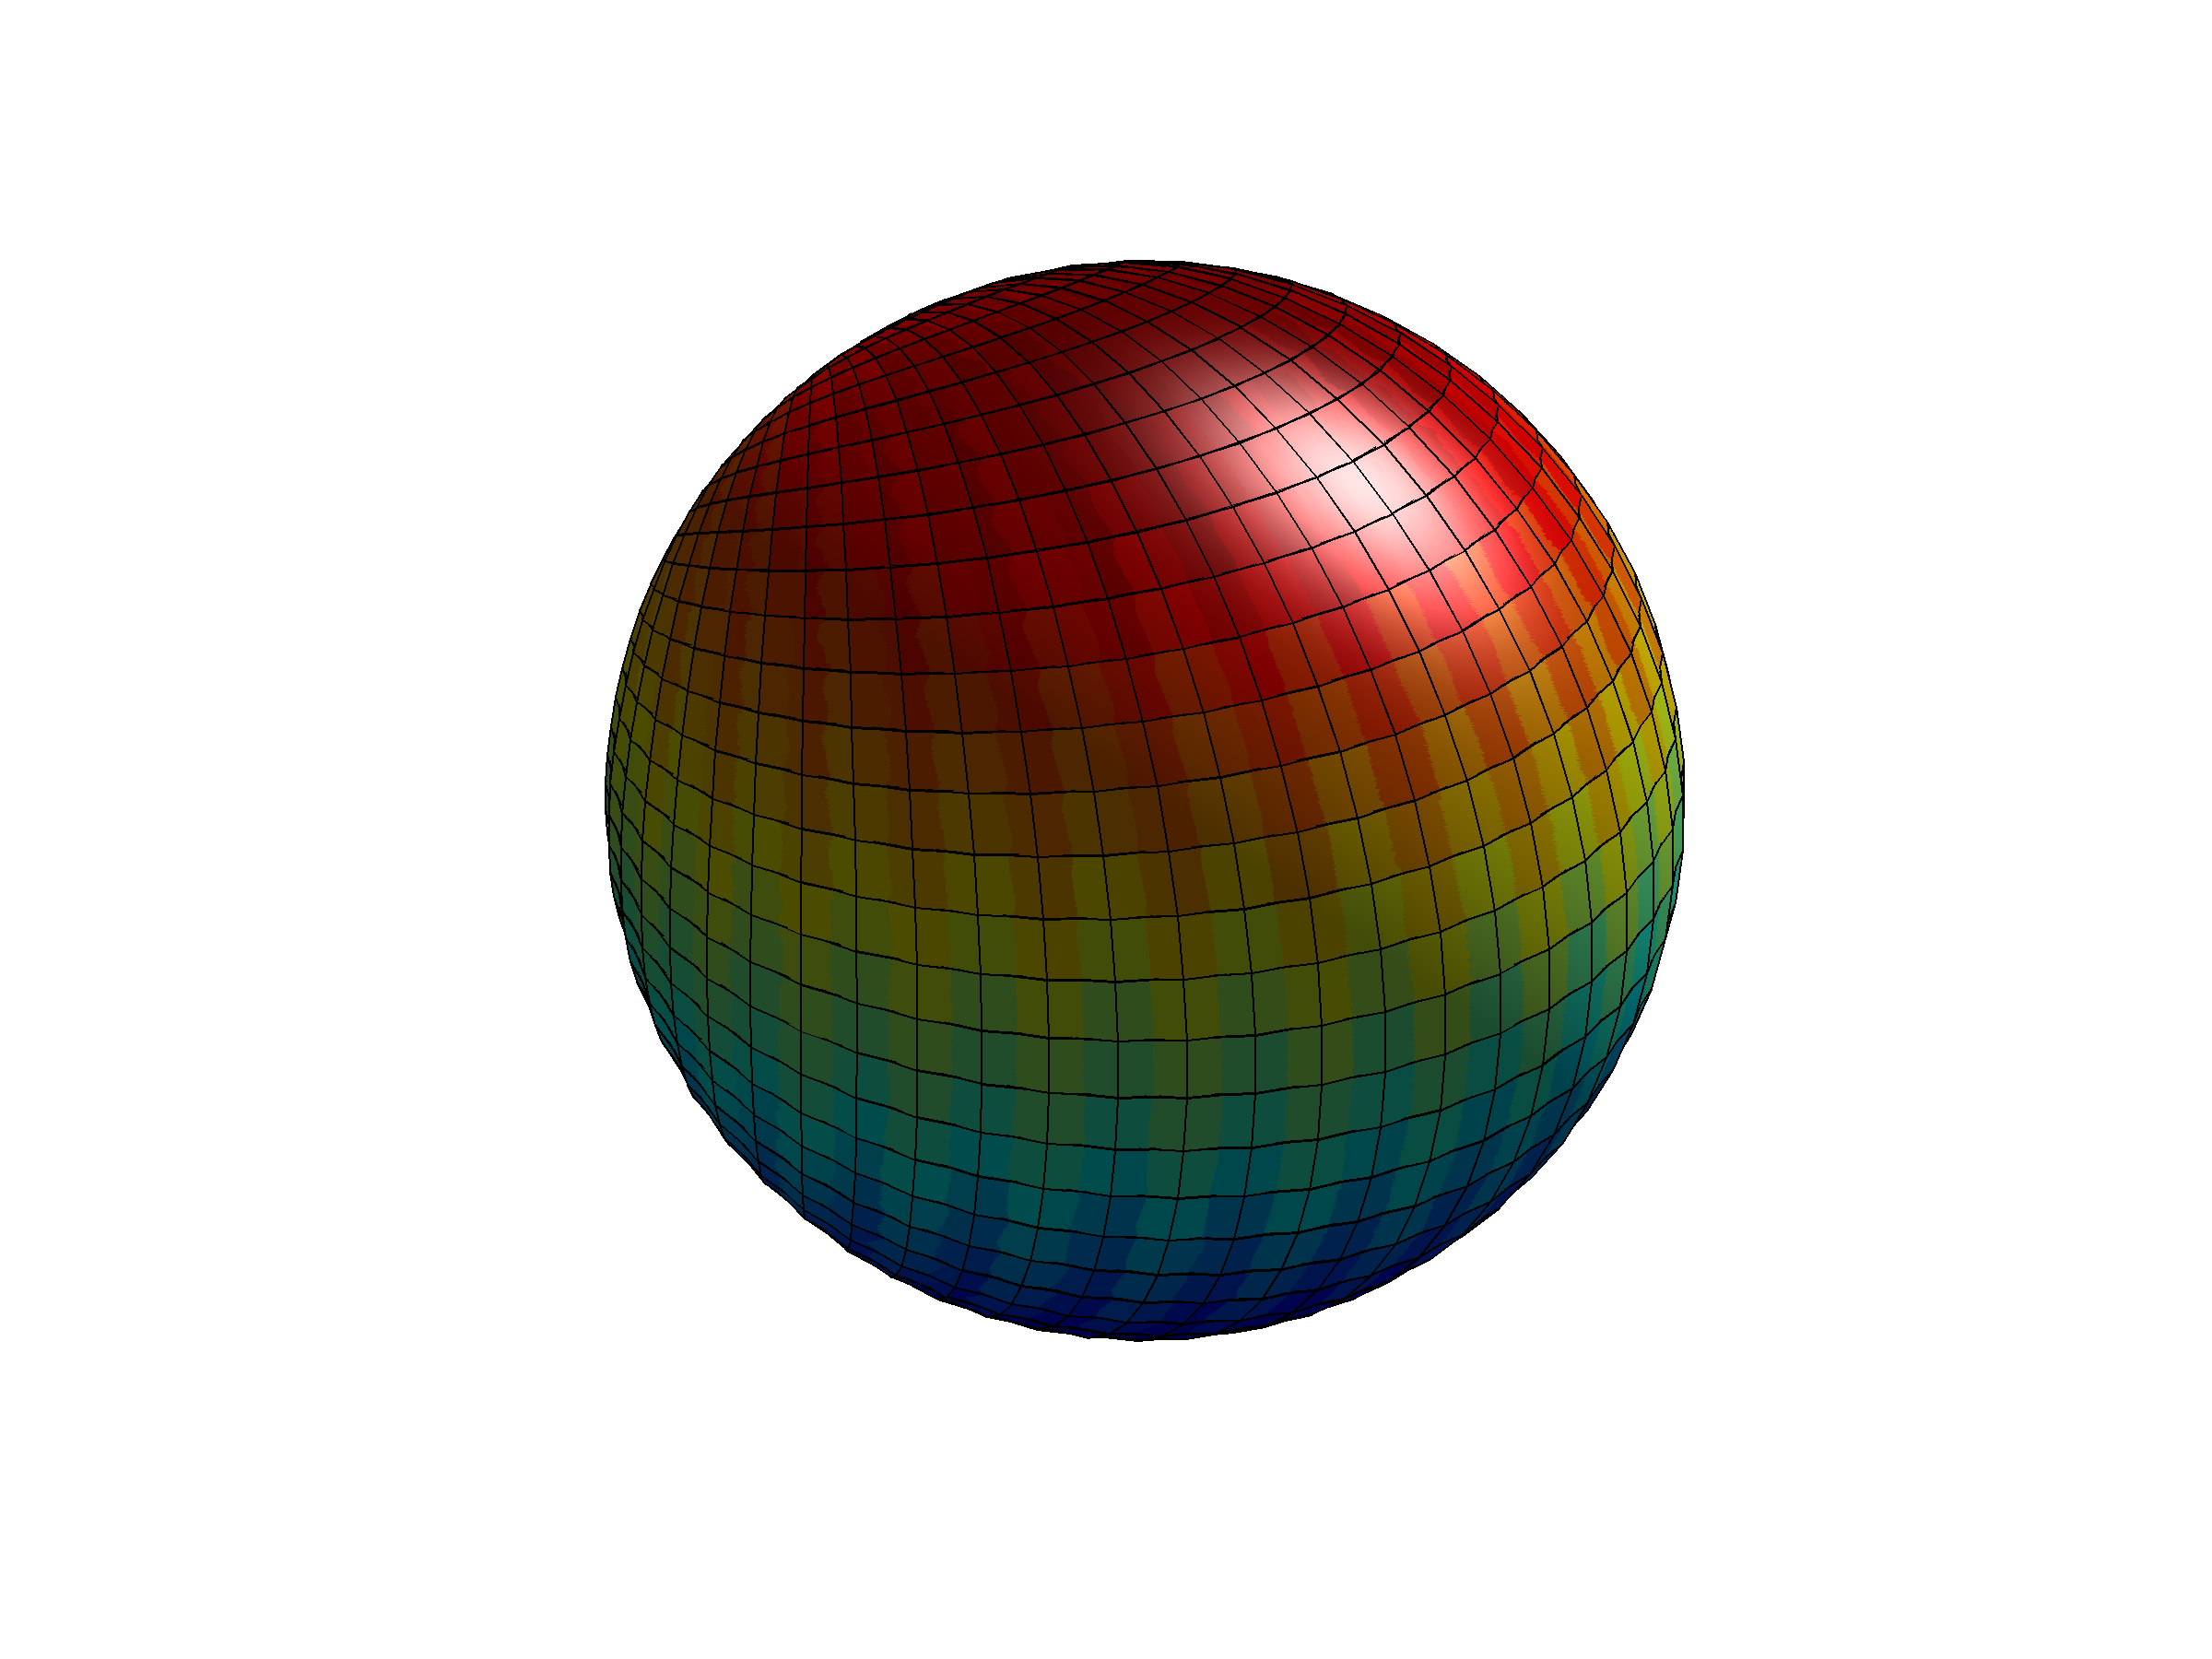
\includegraphics[width=\textwidth]{figures/appendices/Y_1_-1.png}
		\caption{}
	\end{subfigure}
	\hfill
	\begin{subfigure}[b]{0.40\textwidth}
		\centering
		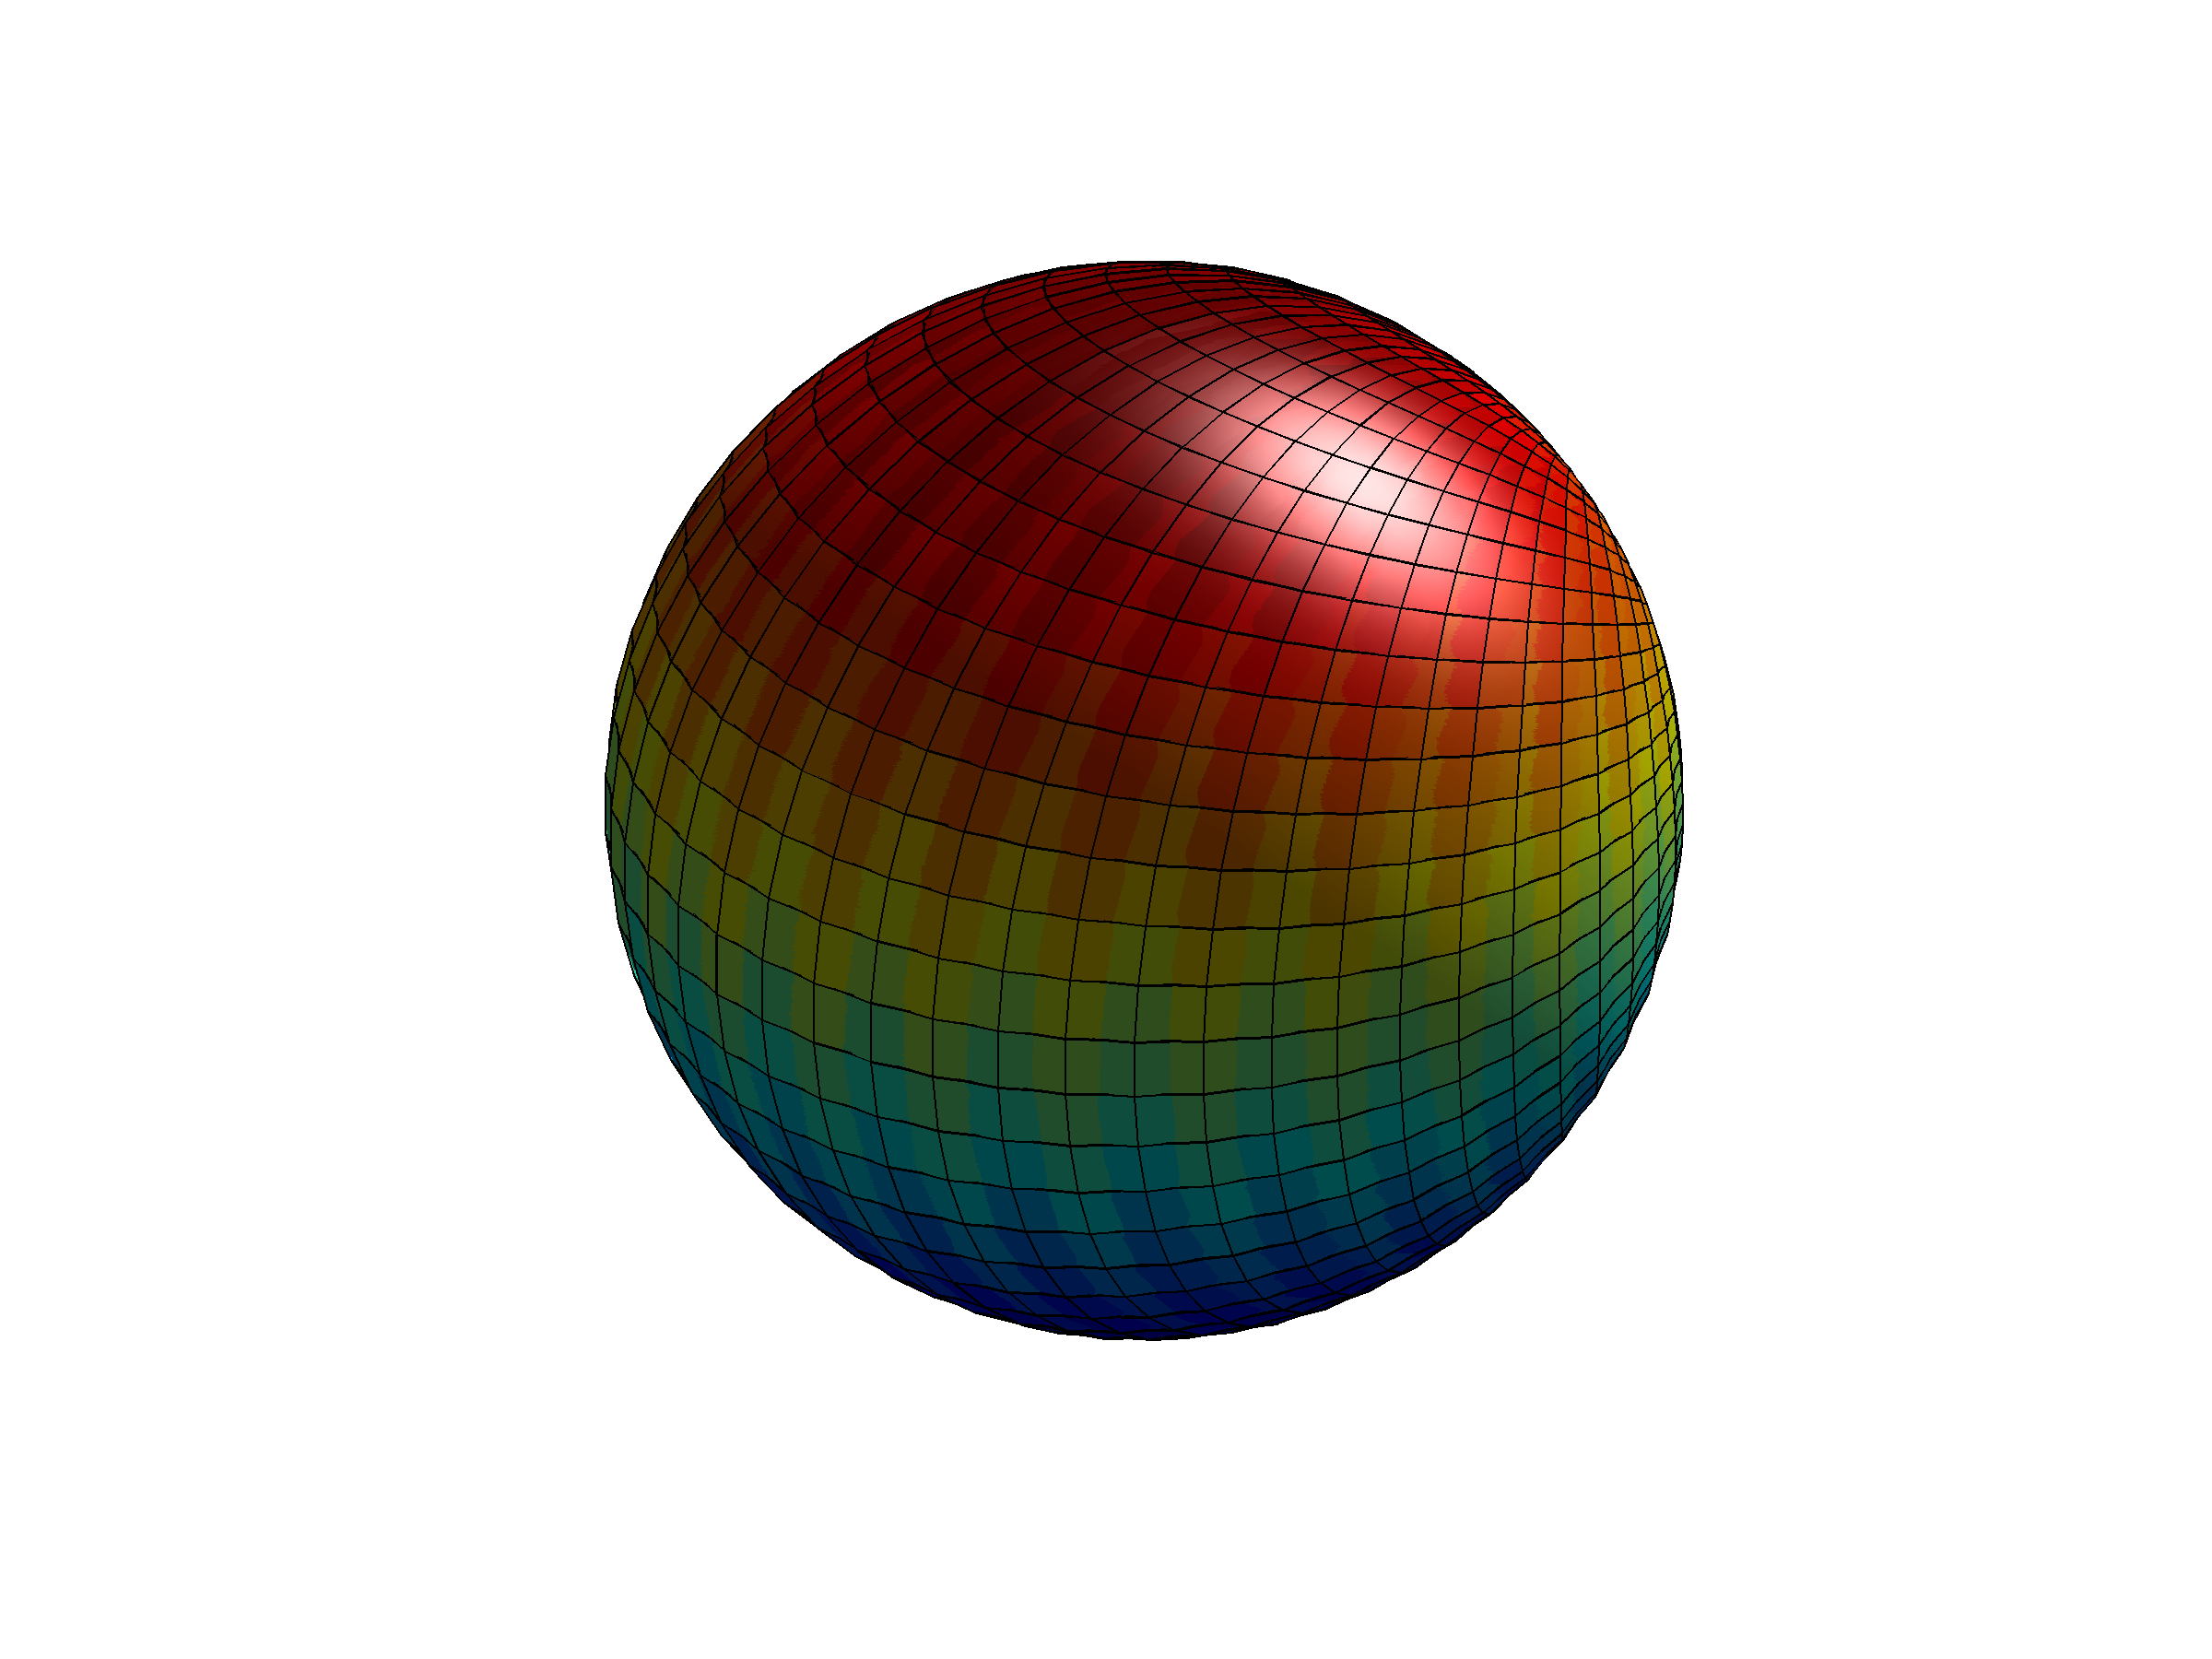
\includegraphics[width=\textwidth]{figures/appendices/Y_1_1.png}
		\caption{}
	\end{subfigure}
\caption{Spherical harmonic functions of degree 1: (a) $Y_{1}^{0}$, (b) $Y_{1}^{-1}$, and (c) $Y_{1}^{1}$.}
\end{figure}

\begin{figure}
\label{fig::Sn_Y2}
\centering
	\begin{subfigure}[b]{0.45\textwidth}
		\centering
		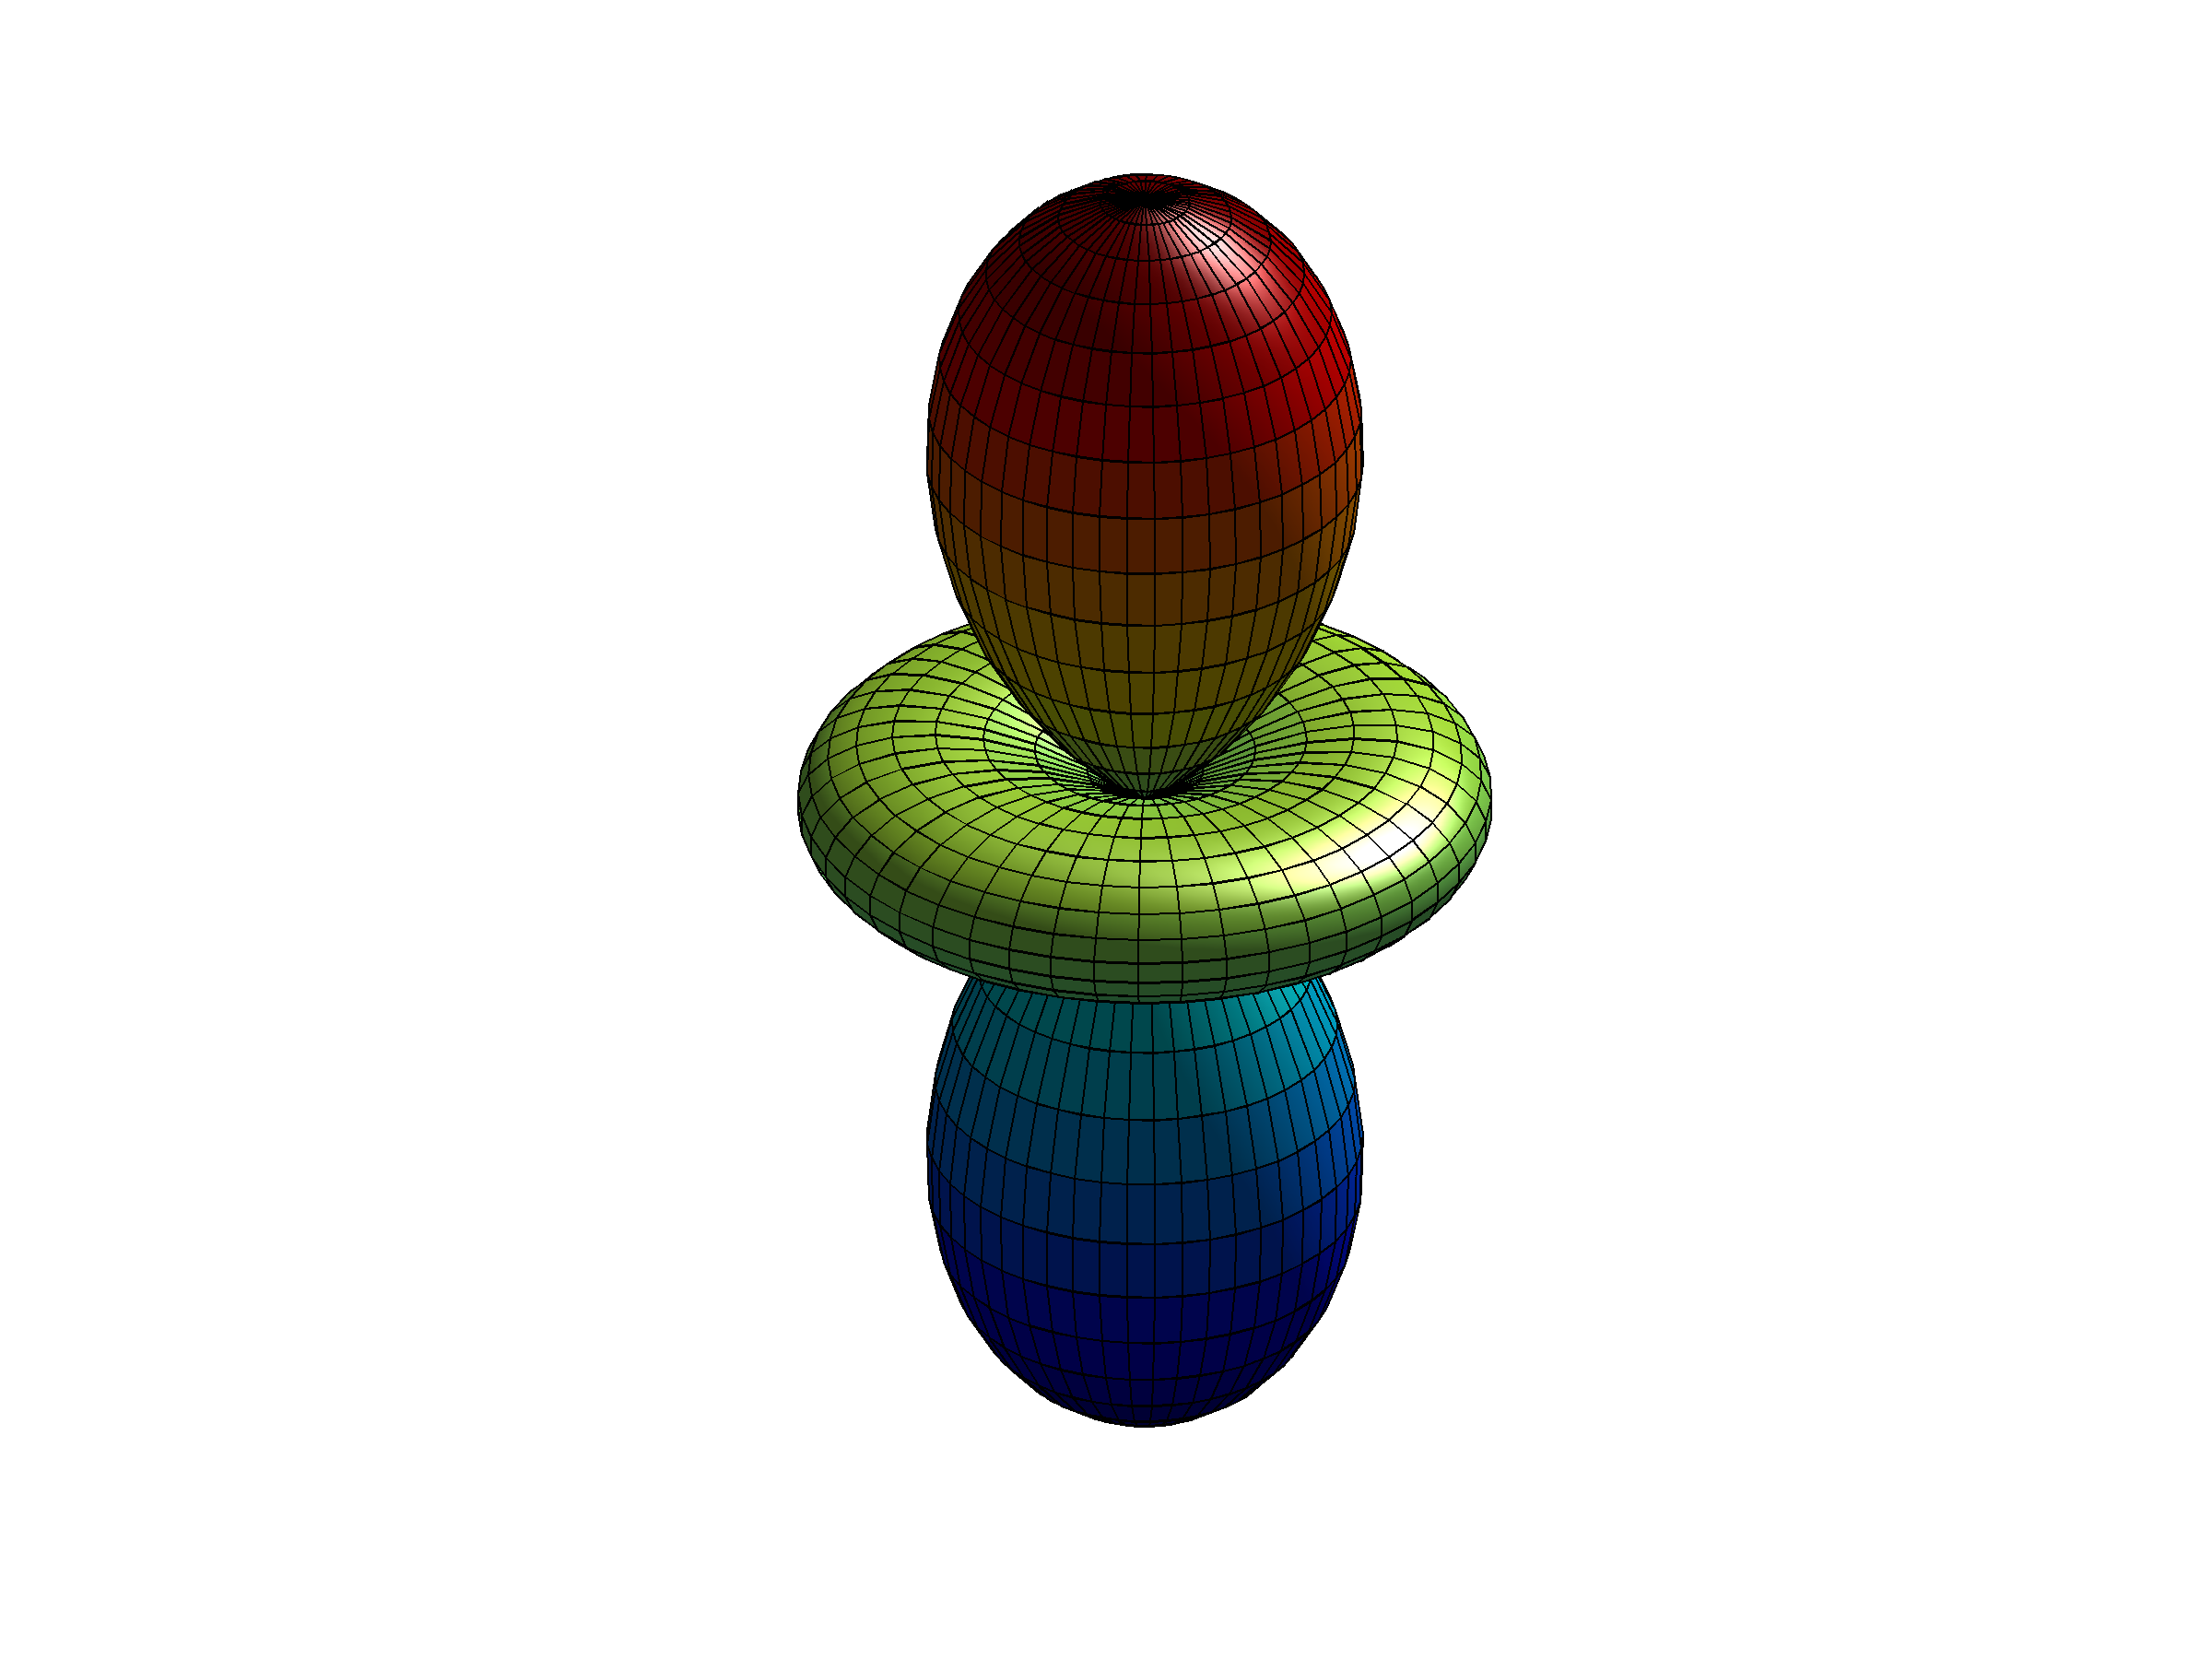
\includegraphics[width=\textwidth]{figures/appendices/Y_2_0.png}
		\caption{}
	\end{subfigure}
	\vfill
	\begin{subfigure}[b]{0.40\textwidth}
		\centering
		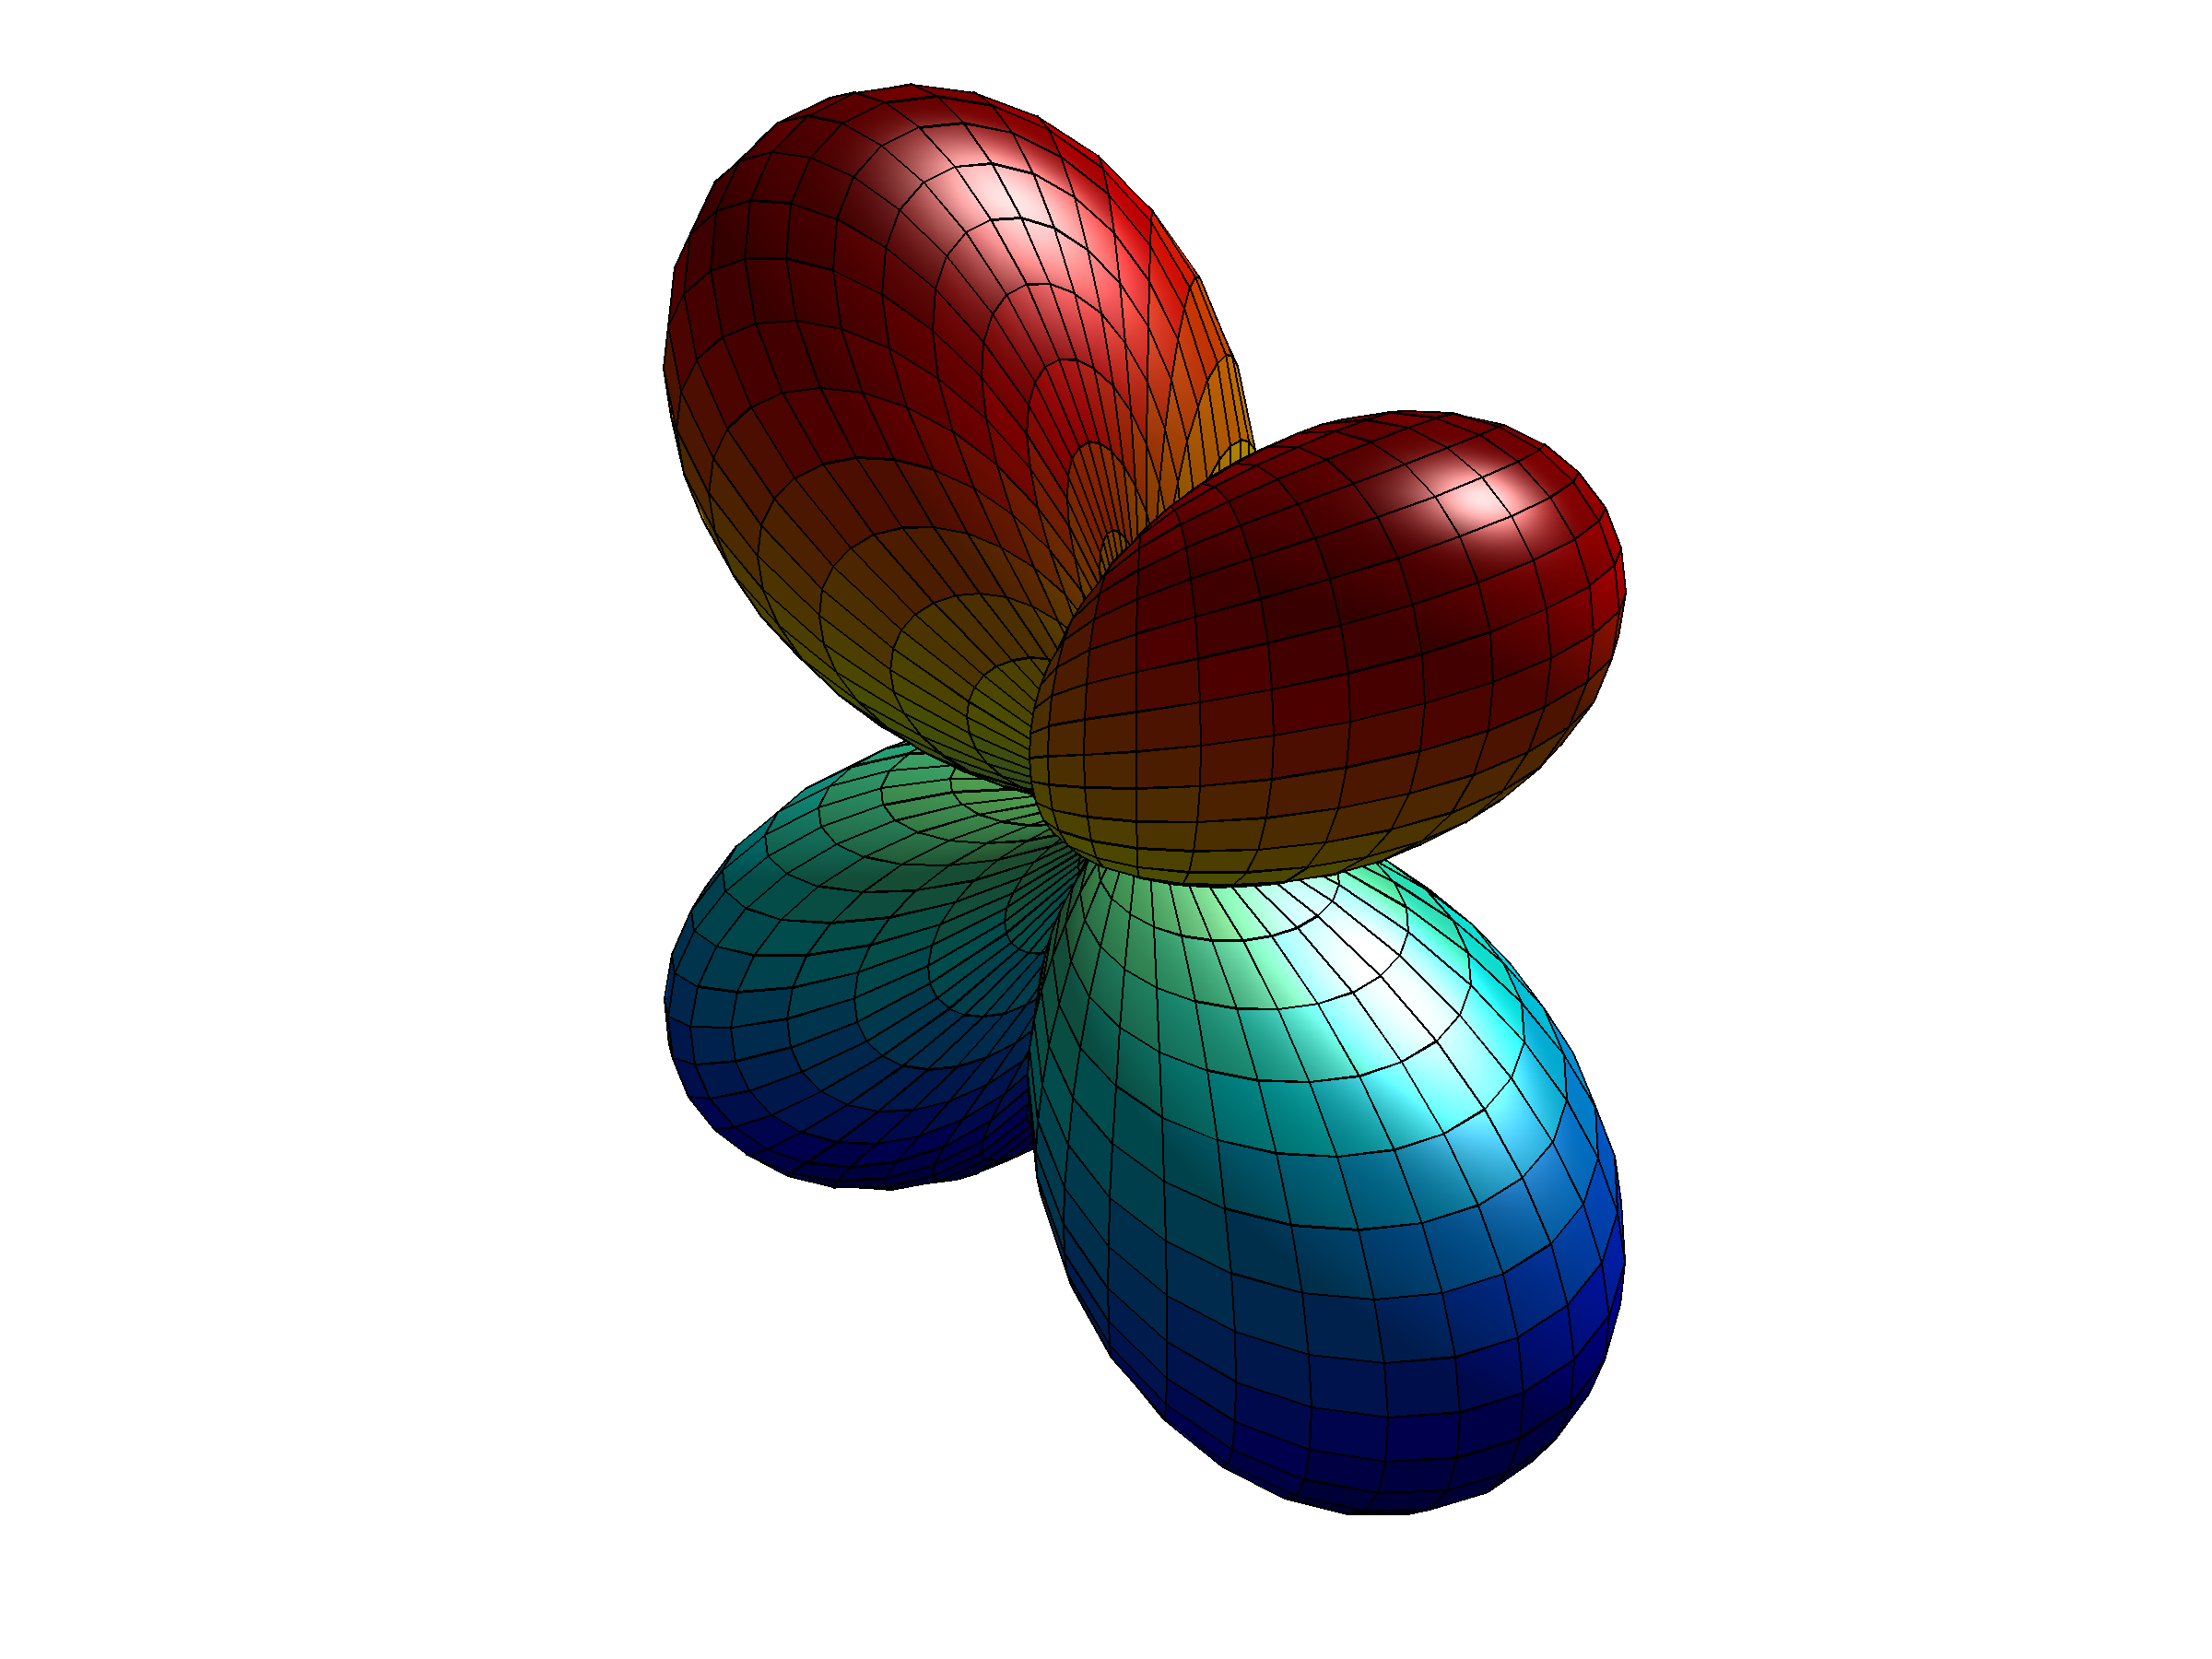
\includegraphics[width=\textwidth]{figures/appendices/Y_2_-1.png}
		\caption{}
	\end{subfigure}
	\hfill
	\begin{subfigure}[b]{0.40\textwidth}
		\centering
		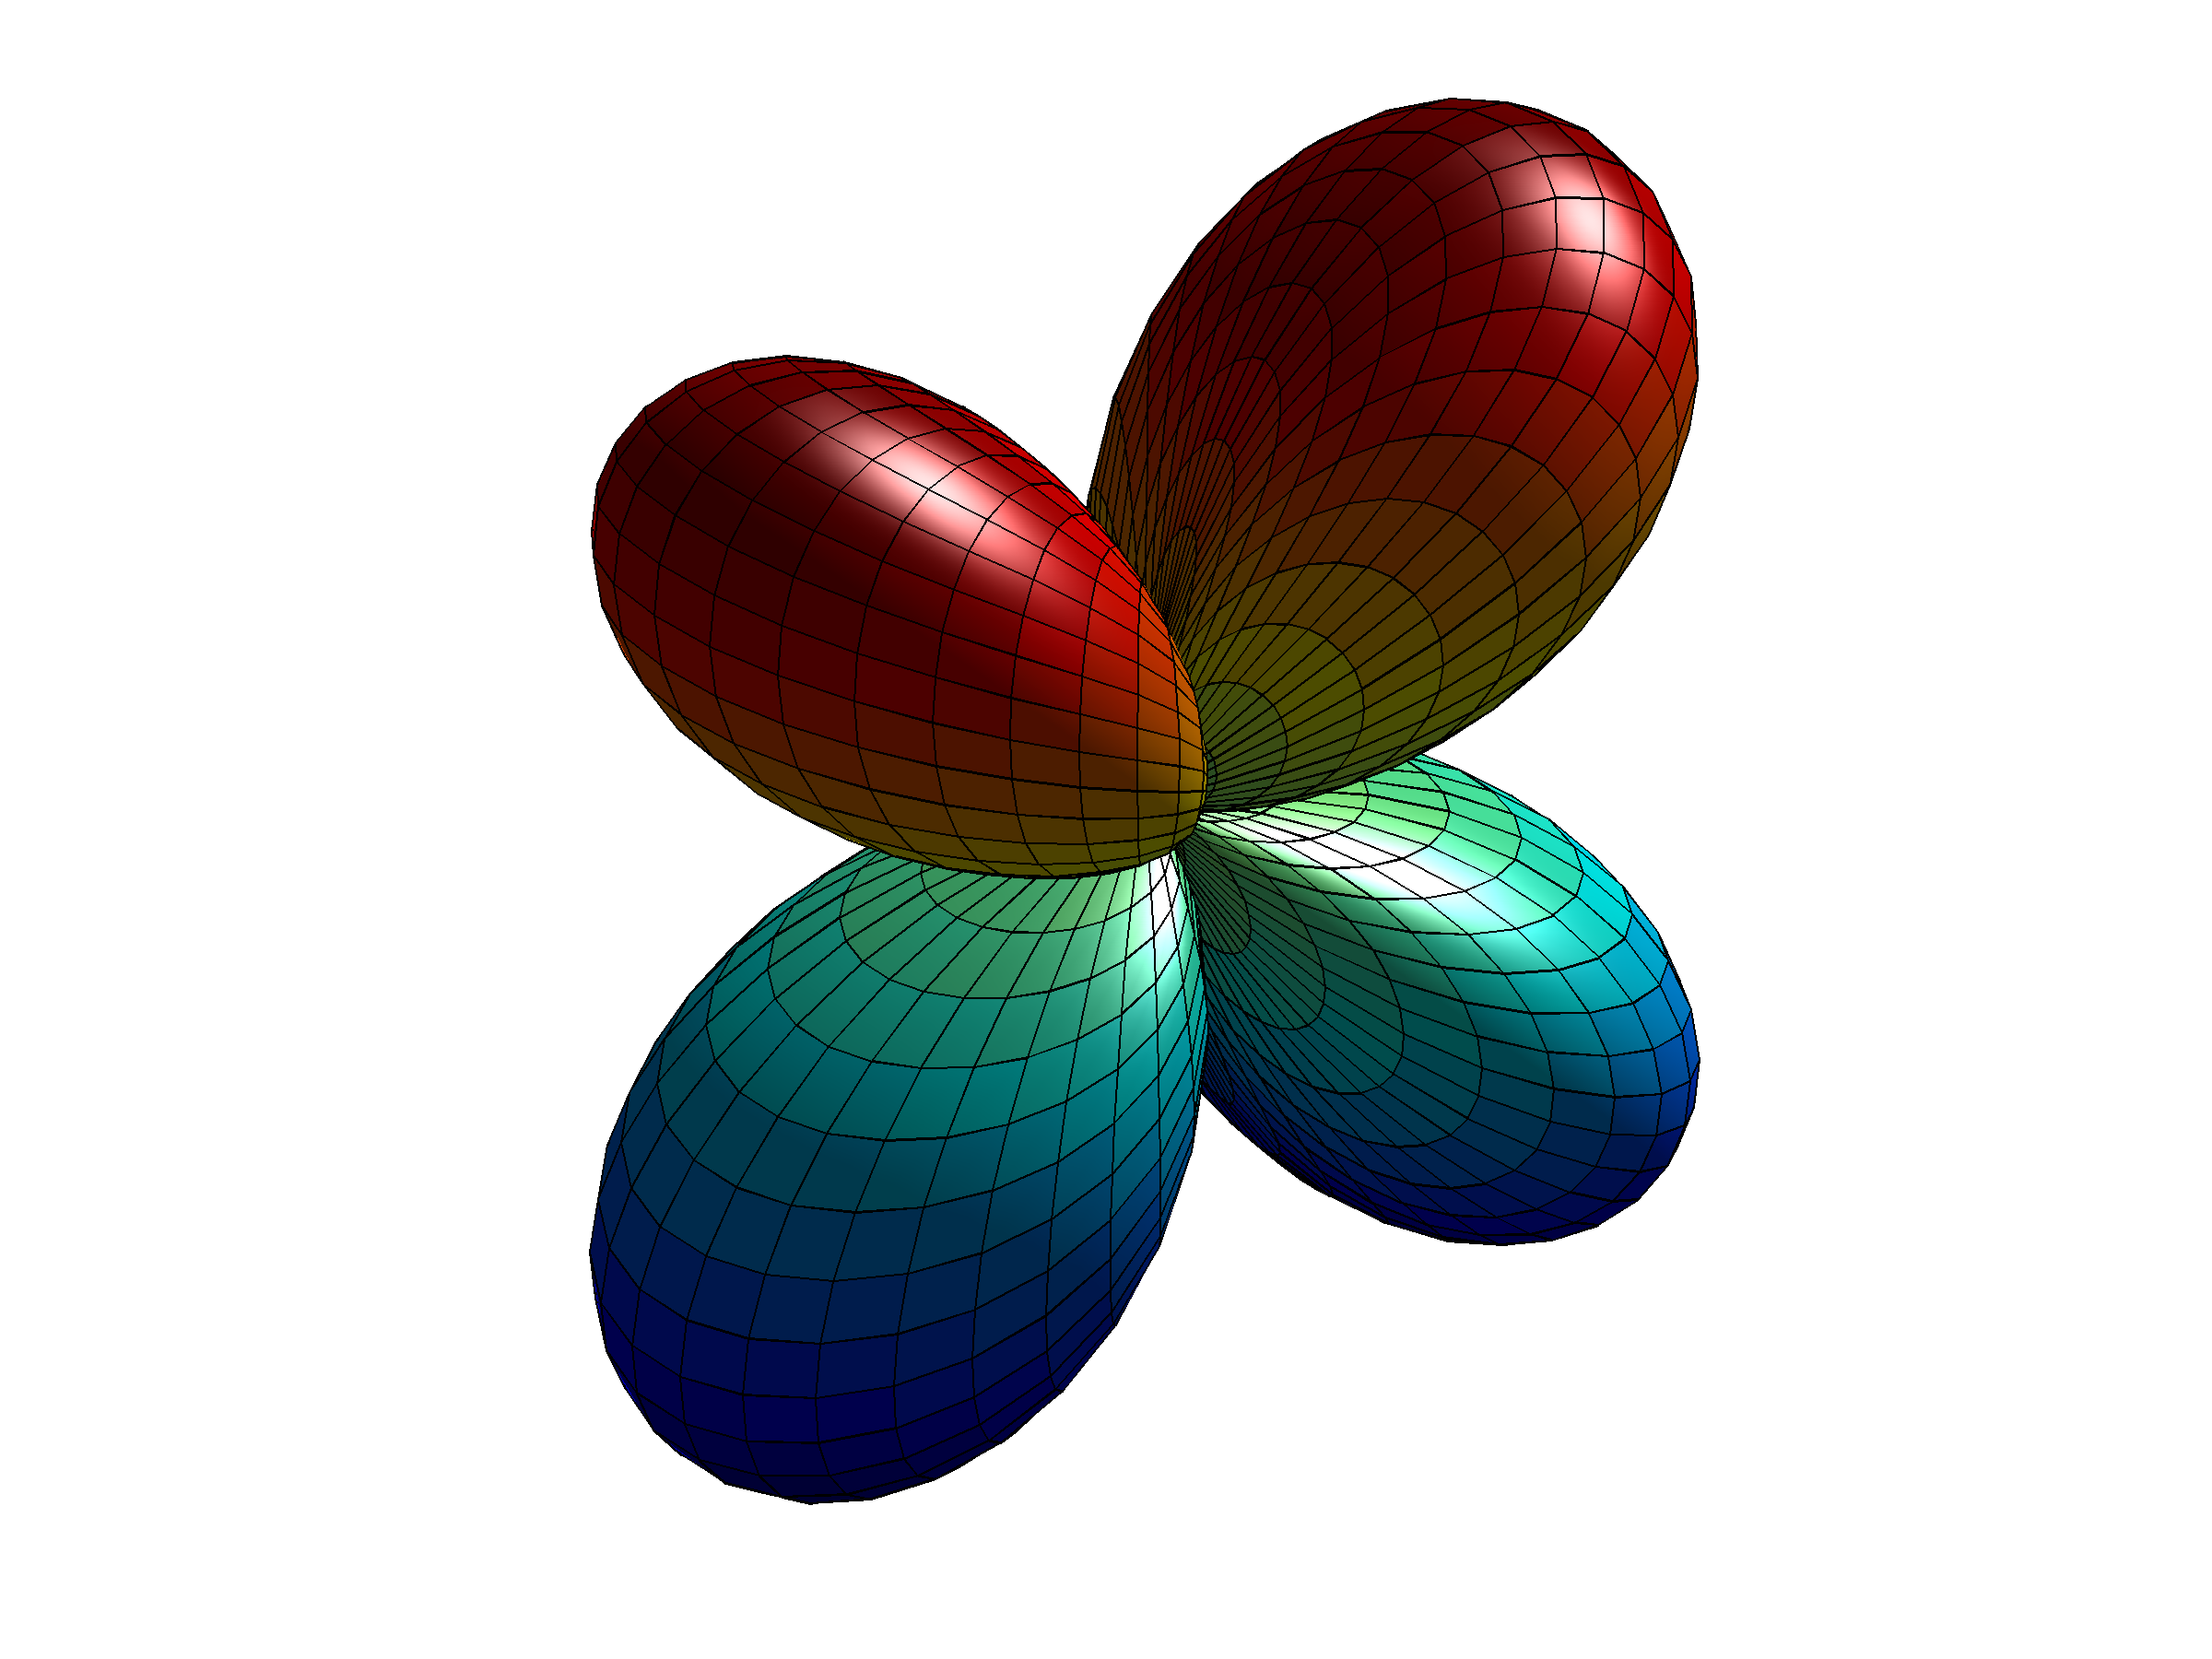
\includegraphics[width=\textwidth]{figures/appendices/Y_2_1.png}
		\caption{}
	\end{subfigure}
	\vfill
	\begin{subfigure}[b]{0.40\textwidth}
		\centering
		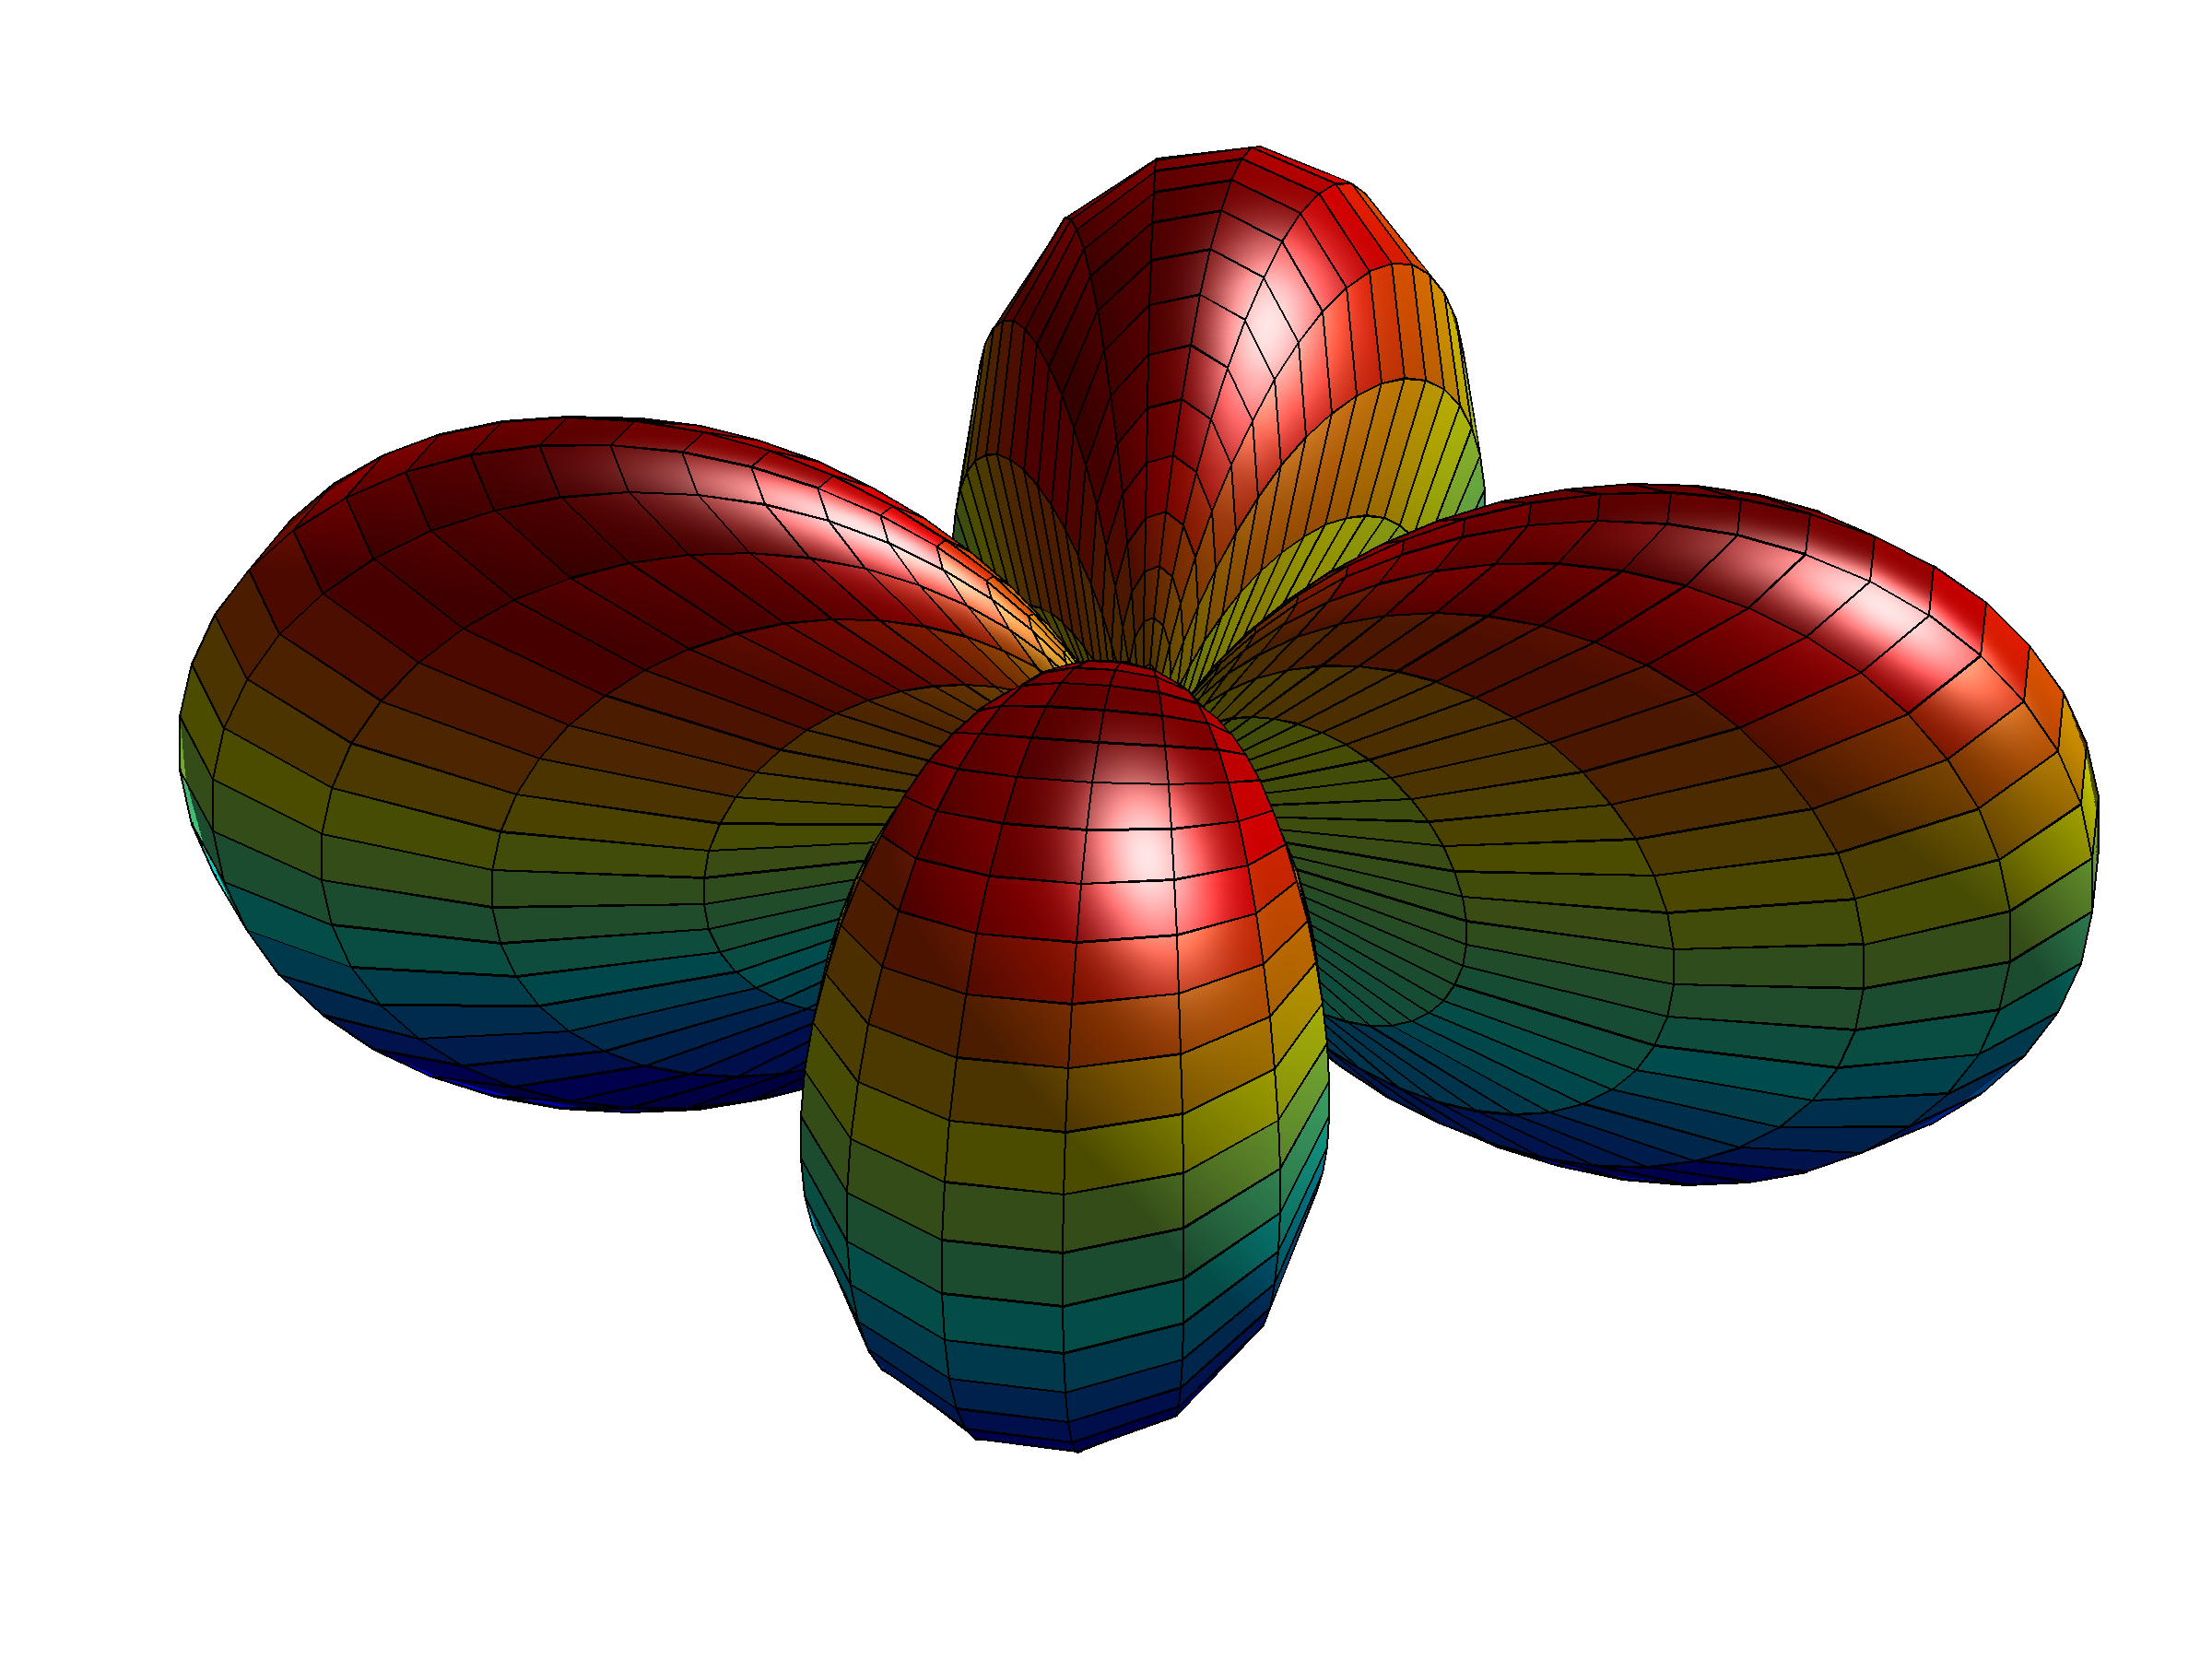
\includegraphics[width=\textwidth]{figures/appendices/Y_2_-2.png}
		\caption{}
	\end{subfigure}
	\hfill
	\begin{subfigure}[b]{0.40\textwidth}
		\centering
		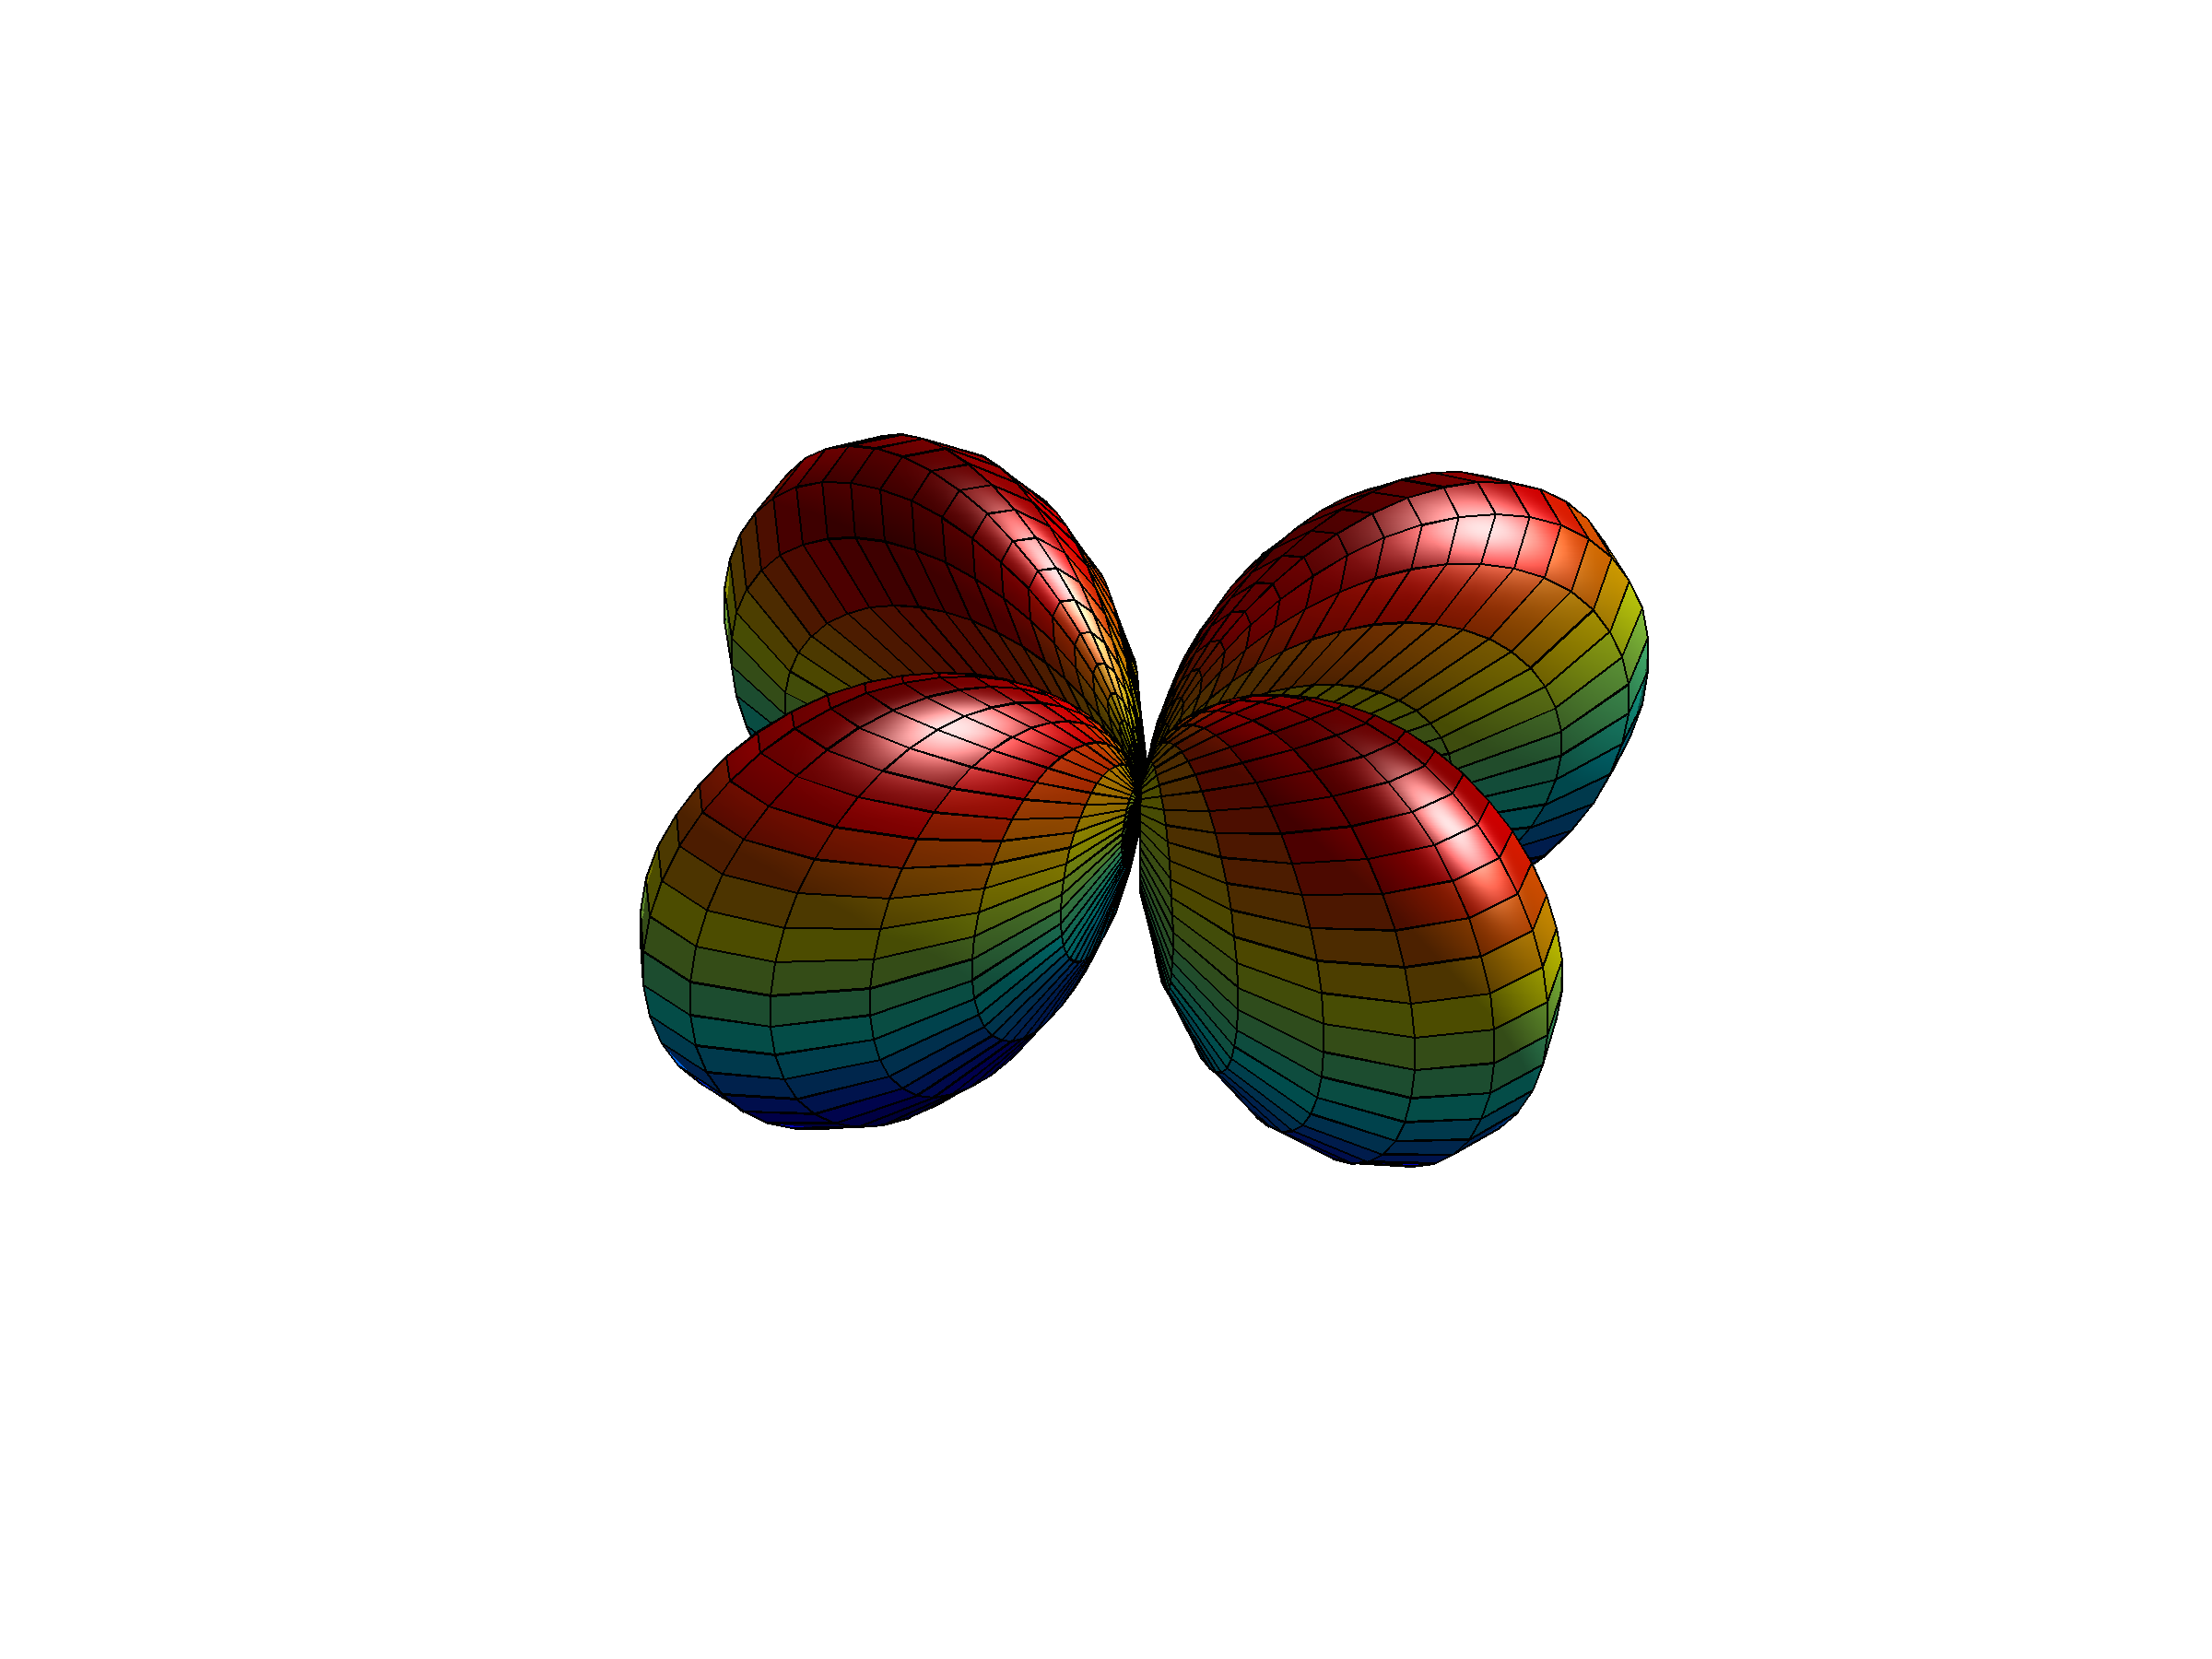
\includegraphics[width=\textwidth]{figures/appendices/Y_2_2.png}
		\caption{}
	\end{subfigure}
\caption{Spherical harmonic functions of degree 2: (a) $Y_{2}^{0}$, (b) $Y_{2}^{-1}$, (c) $Y_{2}^{1}$, (d) $Y_{2}^{-2}$, and (e) $Y_{2}^{2}$.}
\end{figure}

\begin{figure}
\label{fig::Sn_Y3}
\centering
	\begin{subfigure}[b]{0.40\textwidth}
		\centering
		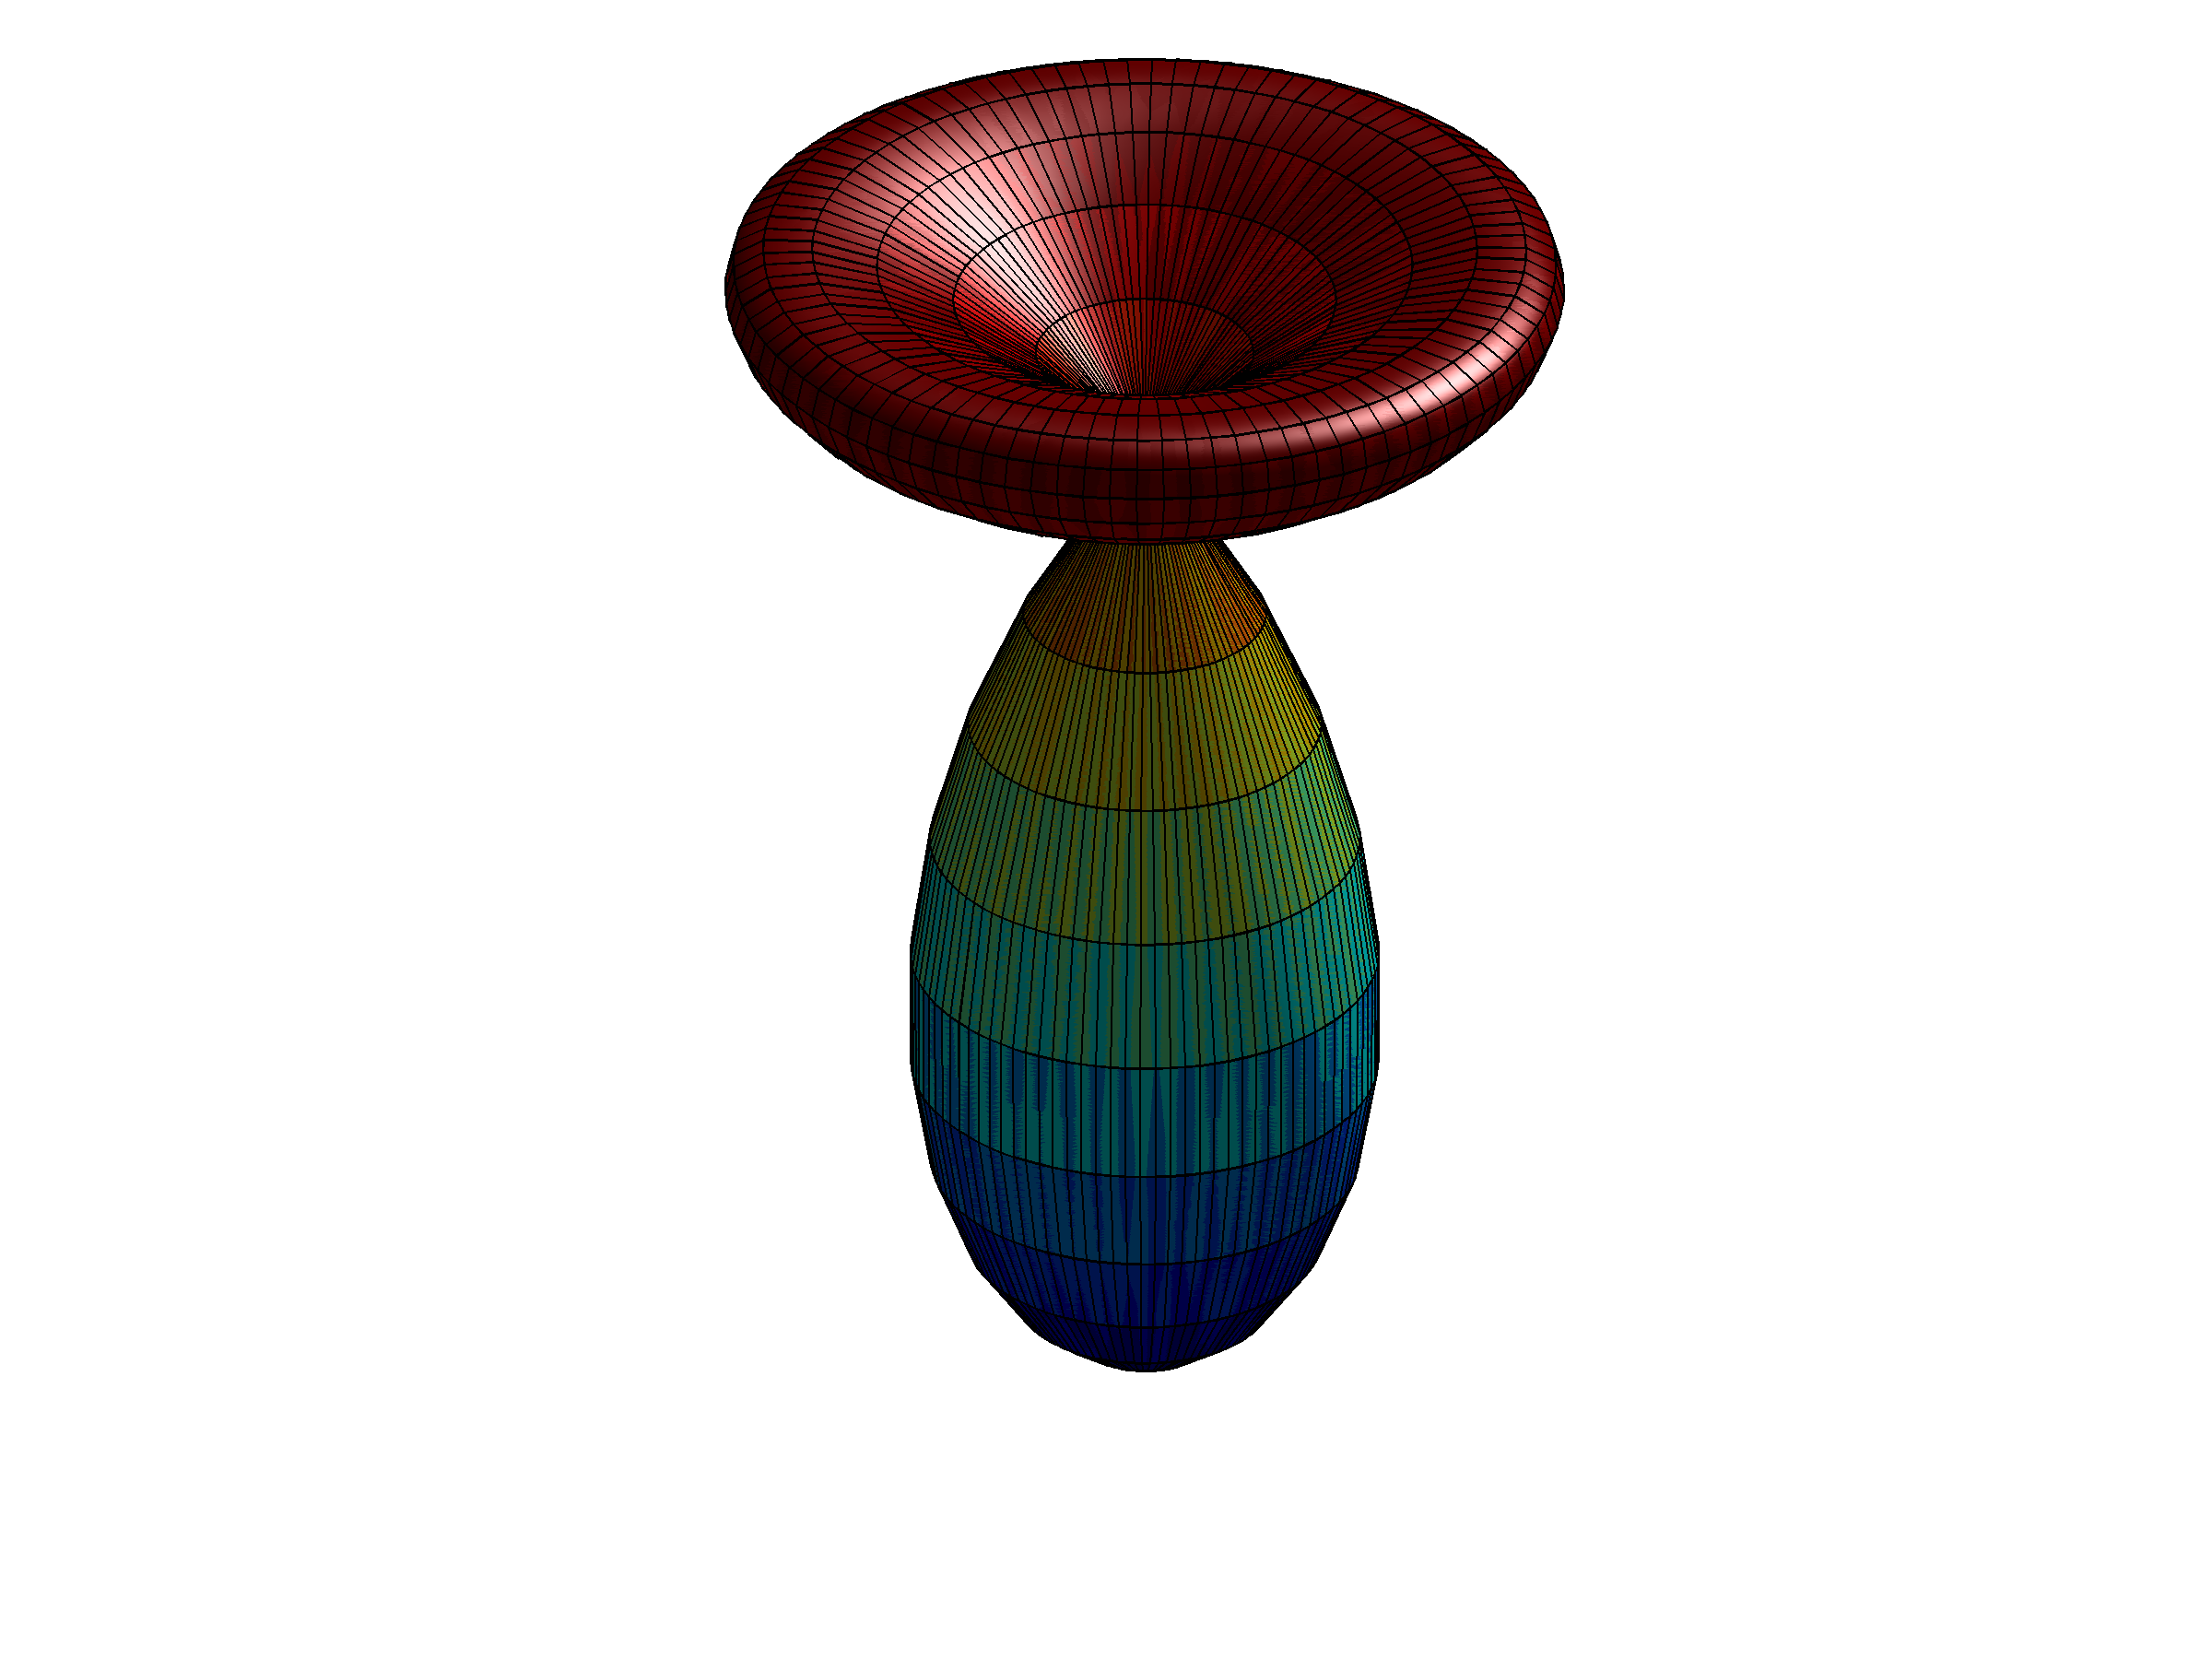
\includegraphics[width=\textwidth]{figures/appendices/Y_3_0.png}
		\caption{}
	\end{subfigure}
	\vfill
	\begin{subfigure}[b]{0.40\textwidth}
		\centering
		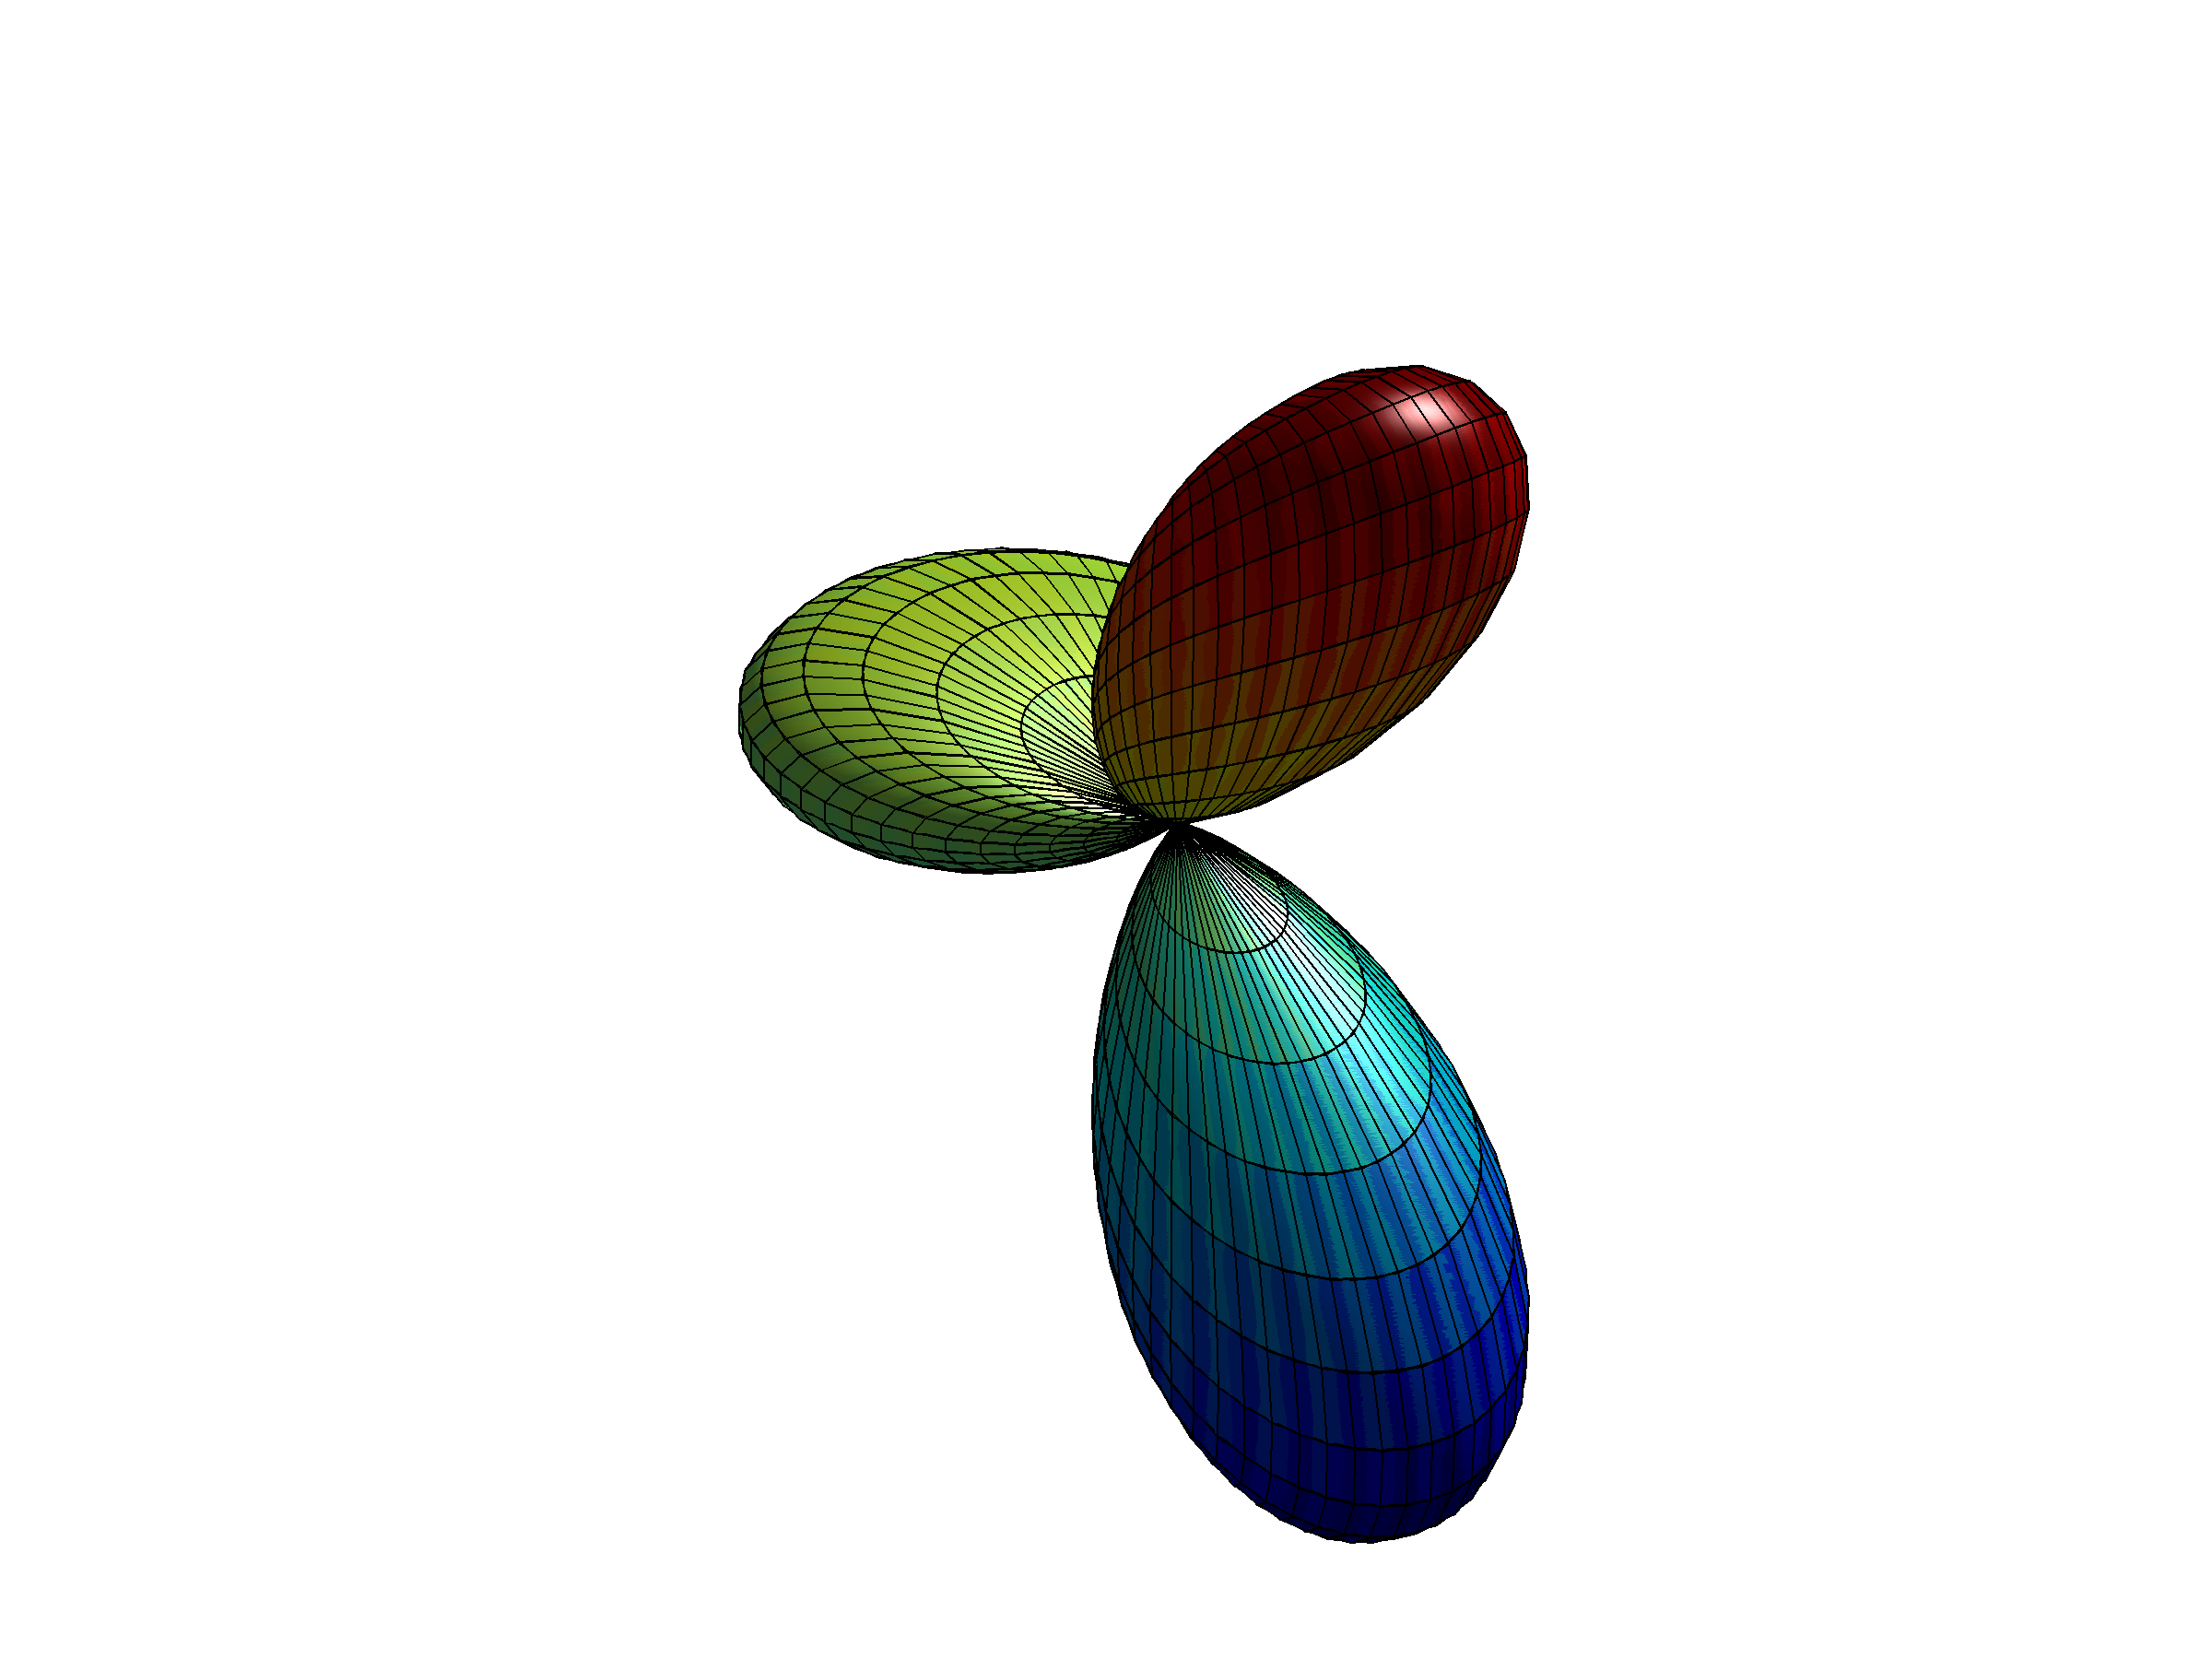
\includegraphics[width=\textwidth]{figures/appendices/Y_3_-1.png}
		\caption{}
	\end{subfigure}
	\hfill
	\begin{subfigure}[b]{0.40\textwidth}
		\centering
		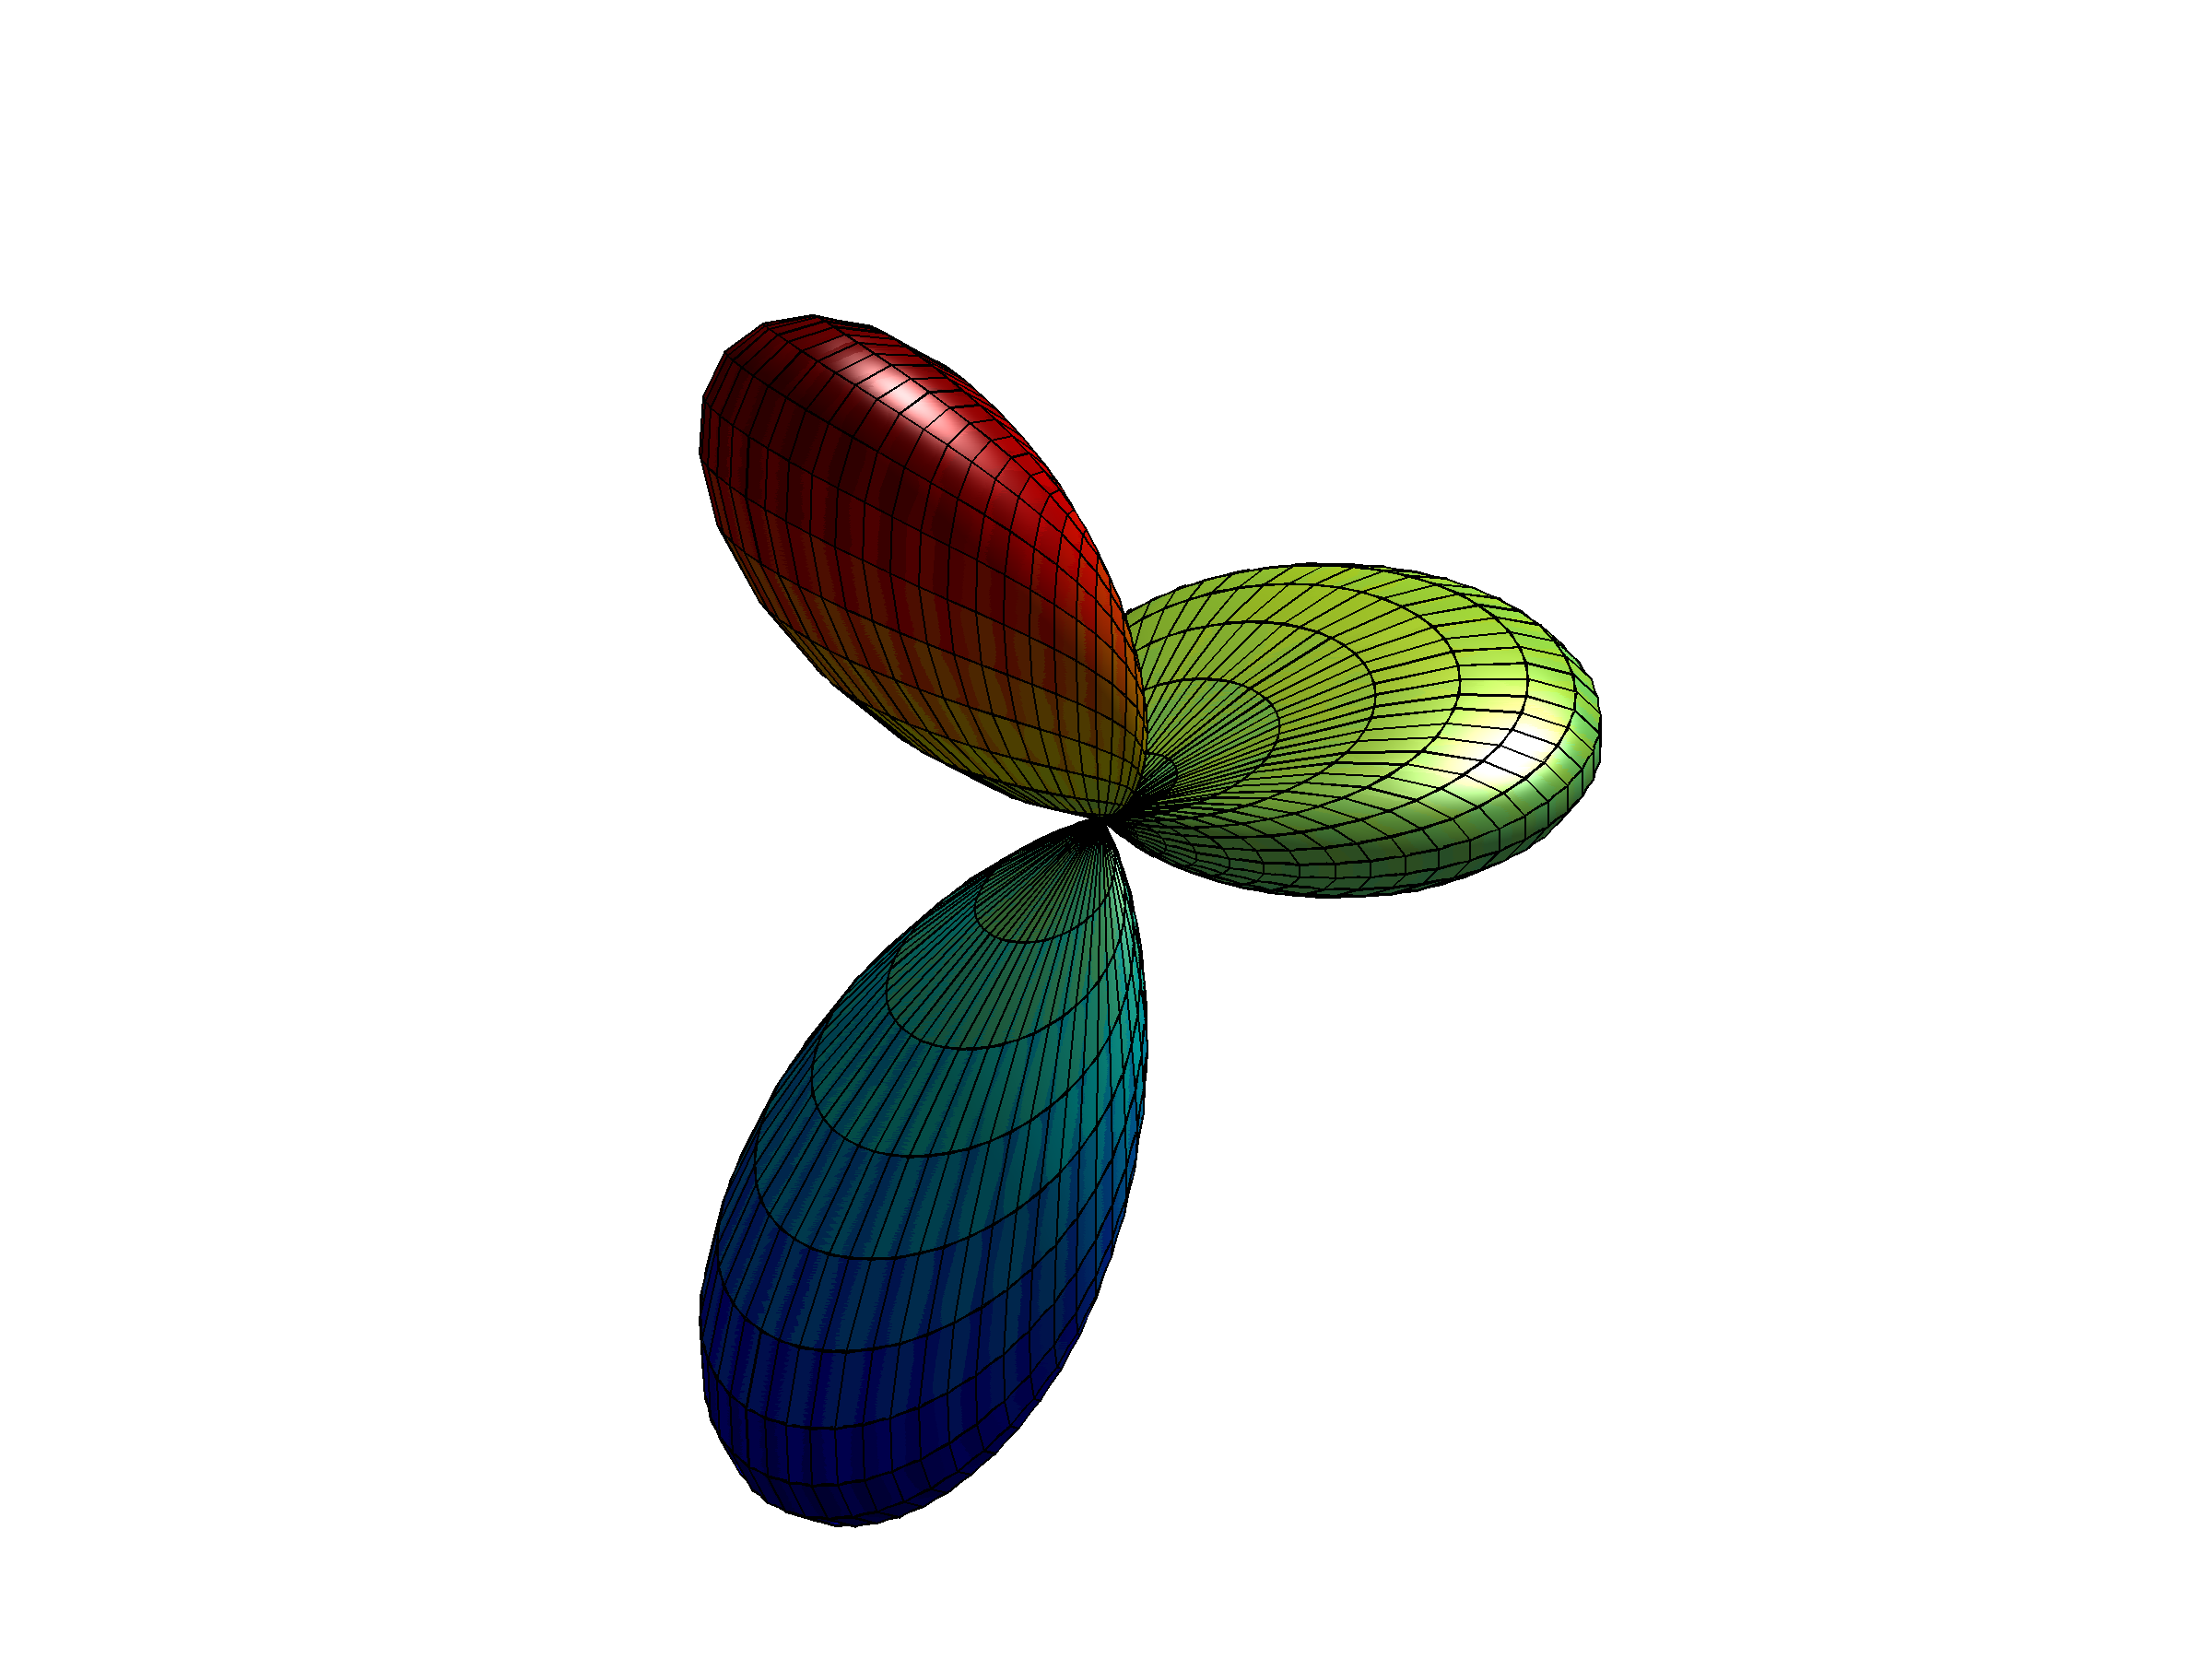
\includegraphics[width=\textwidth]{figures/appendices/Y_3_1.png}
		\caption{}
	\end{subfigure}
	\vfill
	\begin{subfigure}[b]{0.40\textwidth}
		\centering
		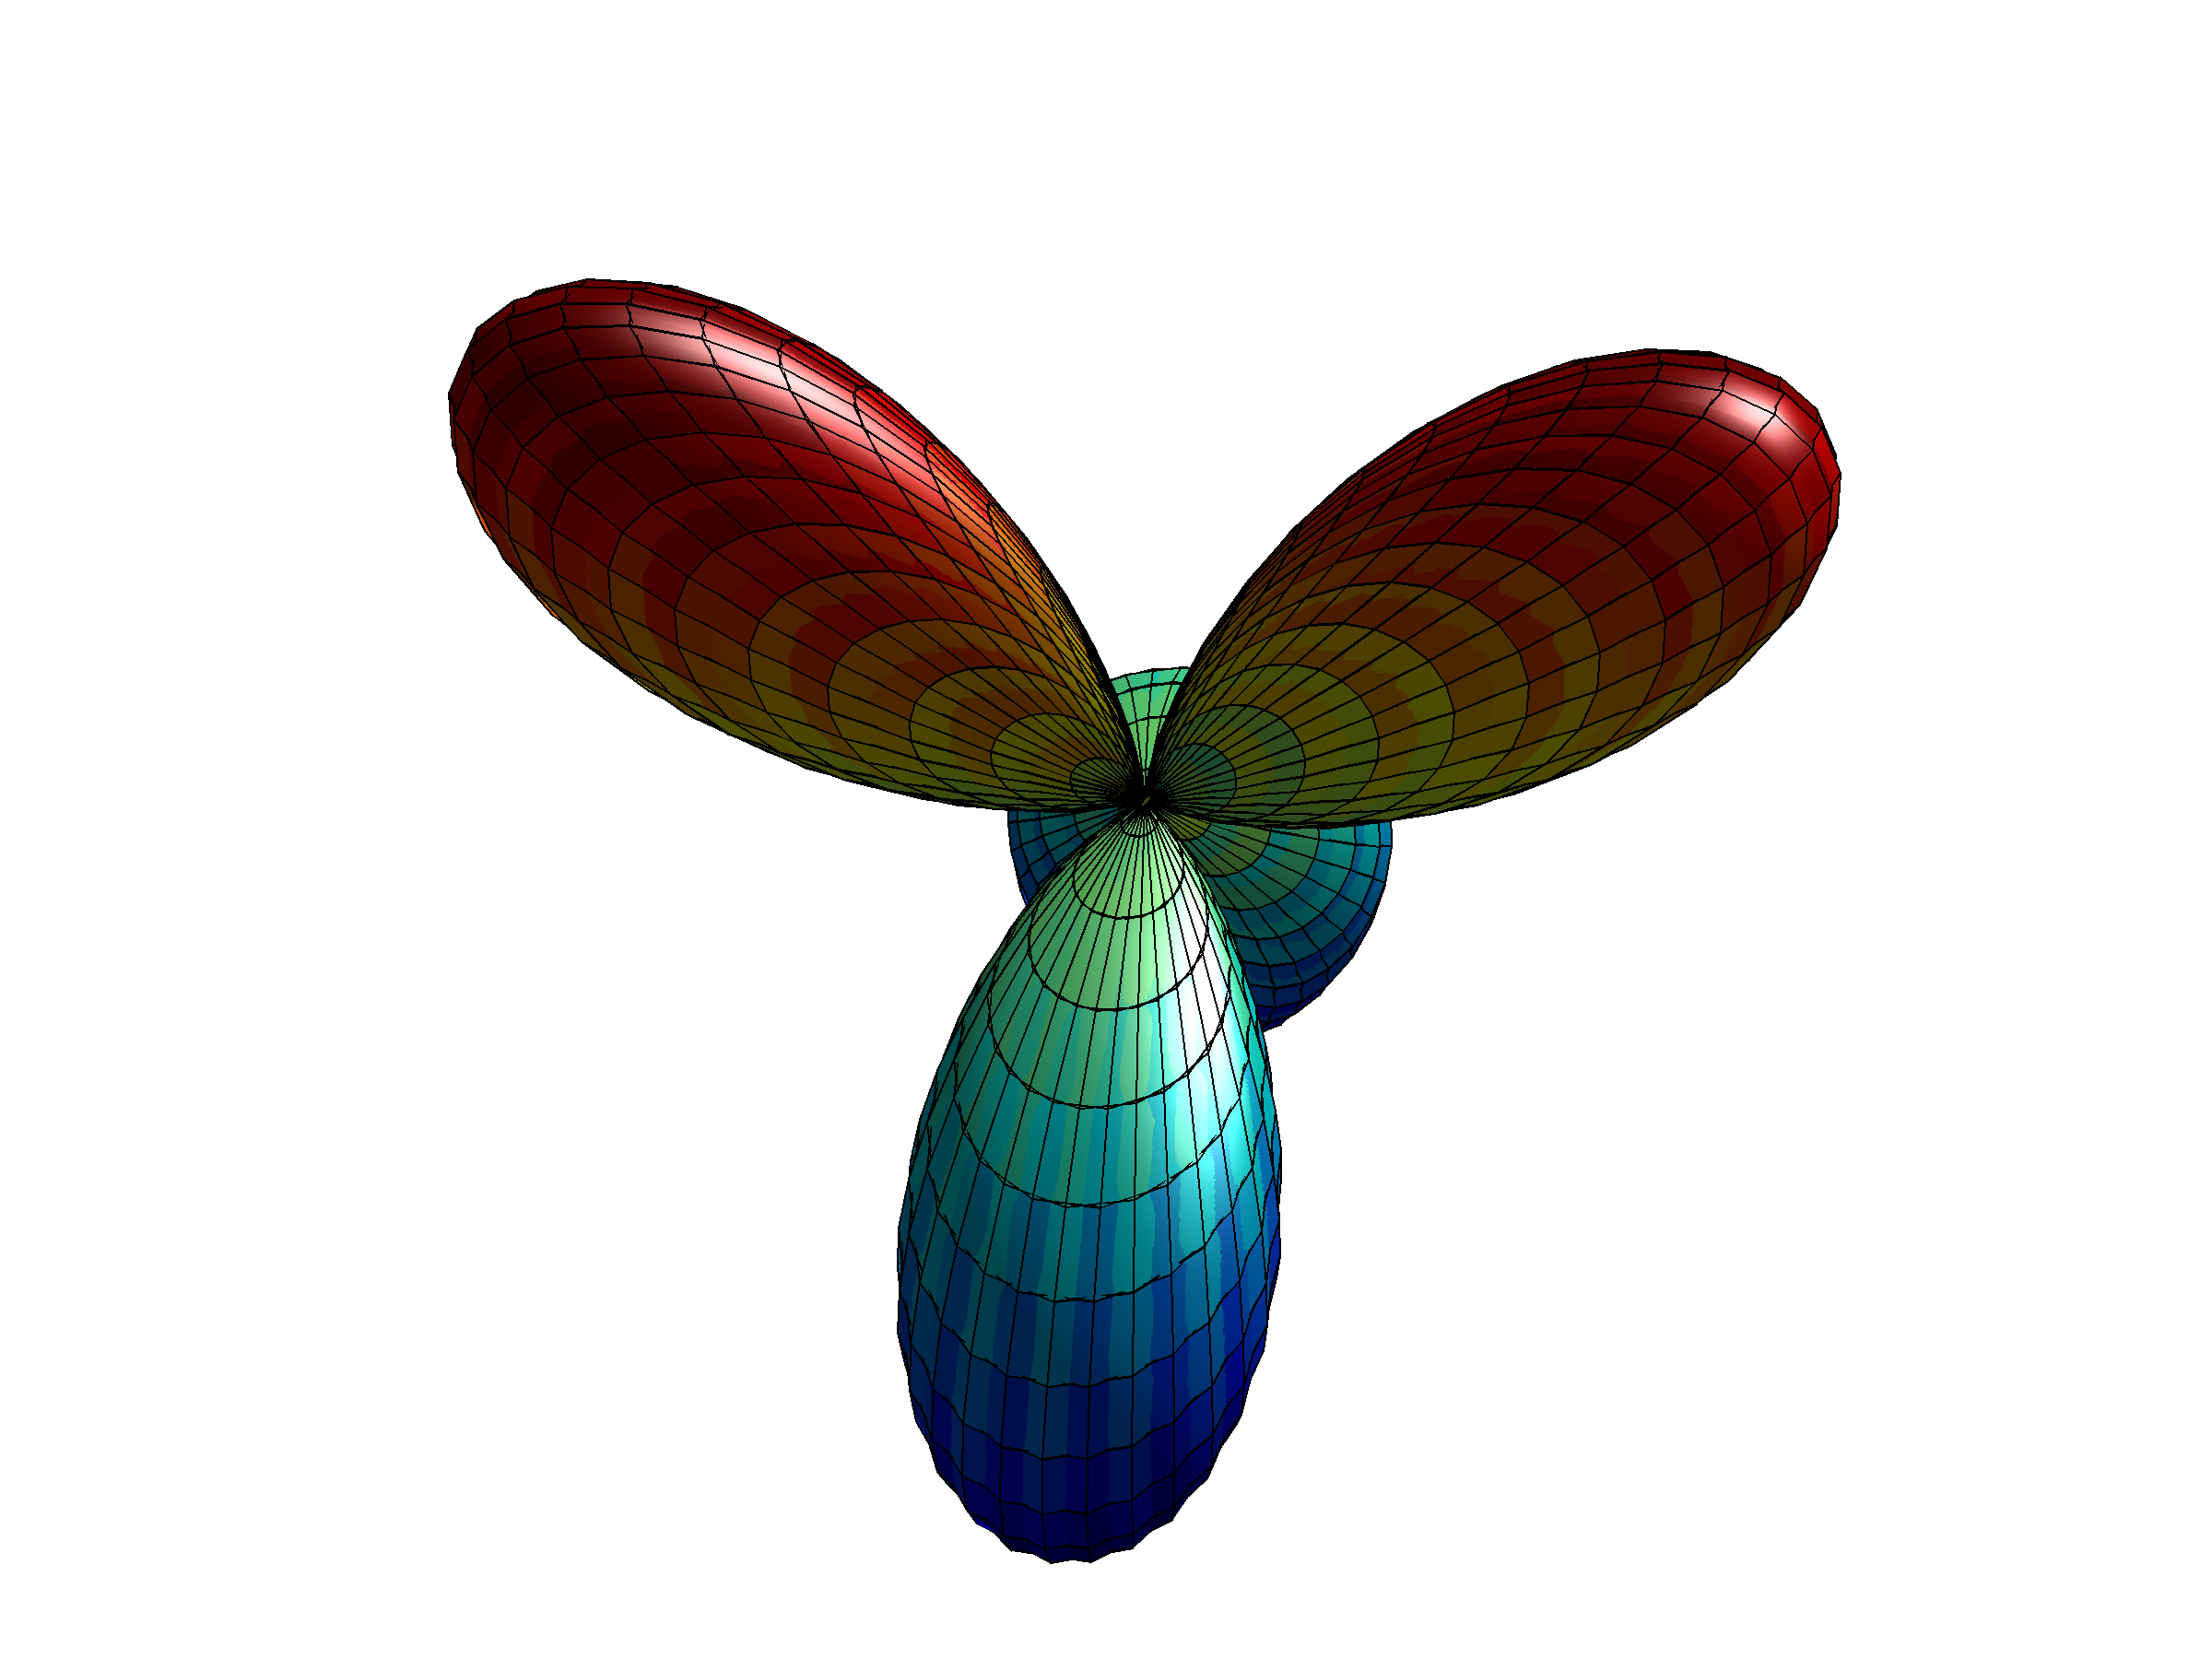
\includegraphics[width=\textwidth]{figures/appendices/Y_3_-2.png}
		\caption{}
	\end{subfigure}
	\hfill
	\begin{subfigure}[b]{0.40\textwidth}
		\centering
		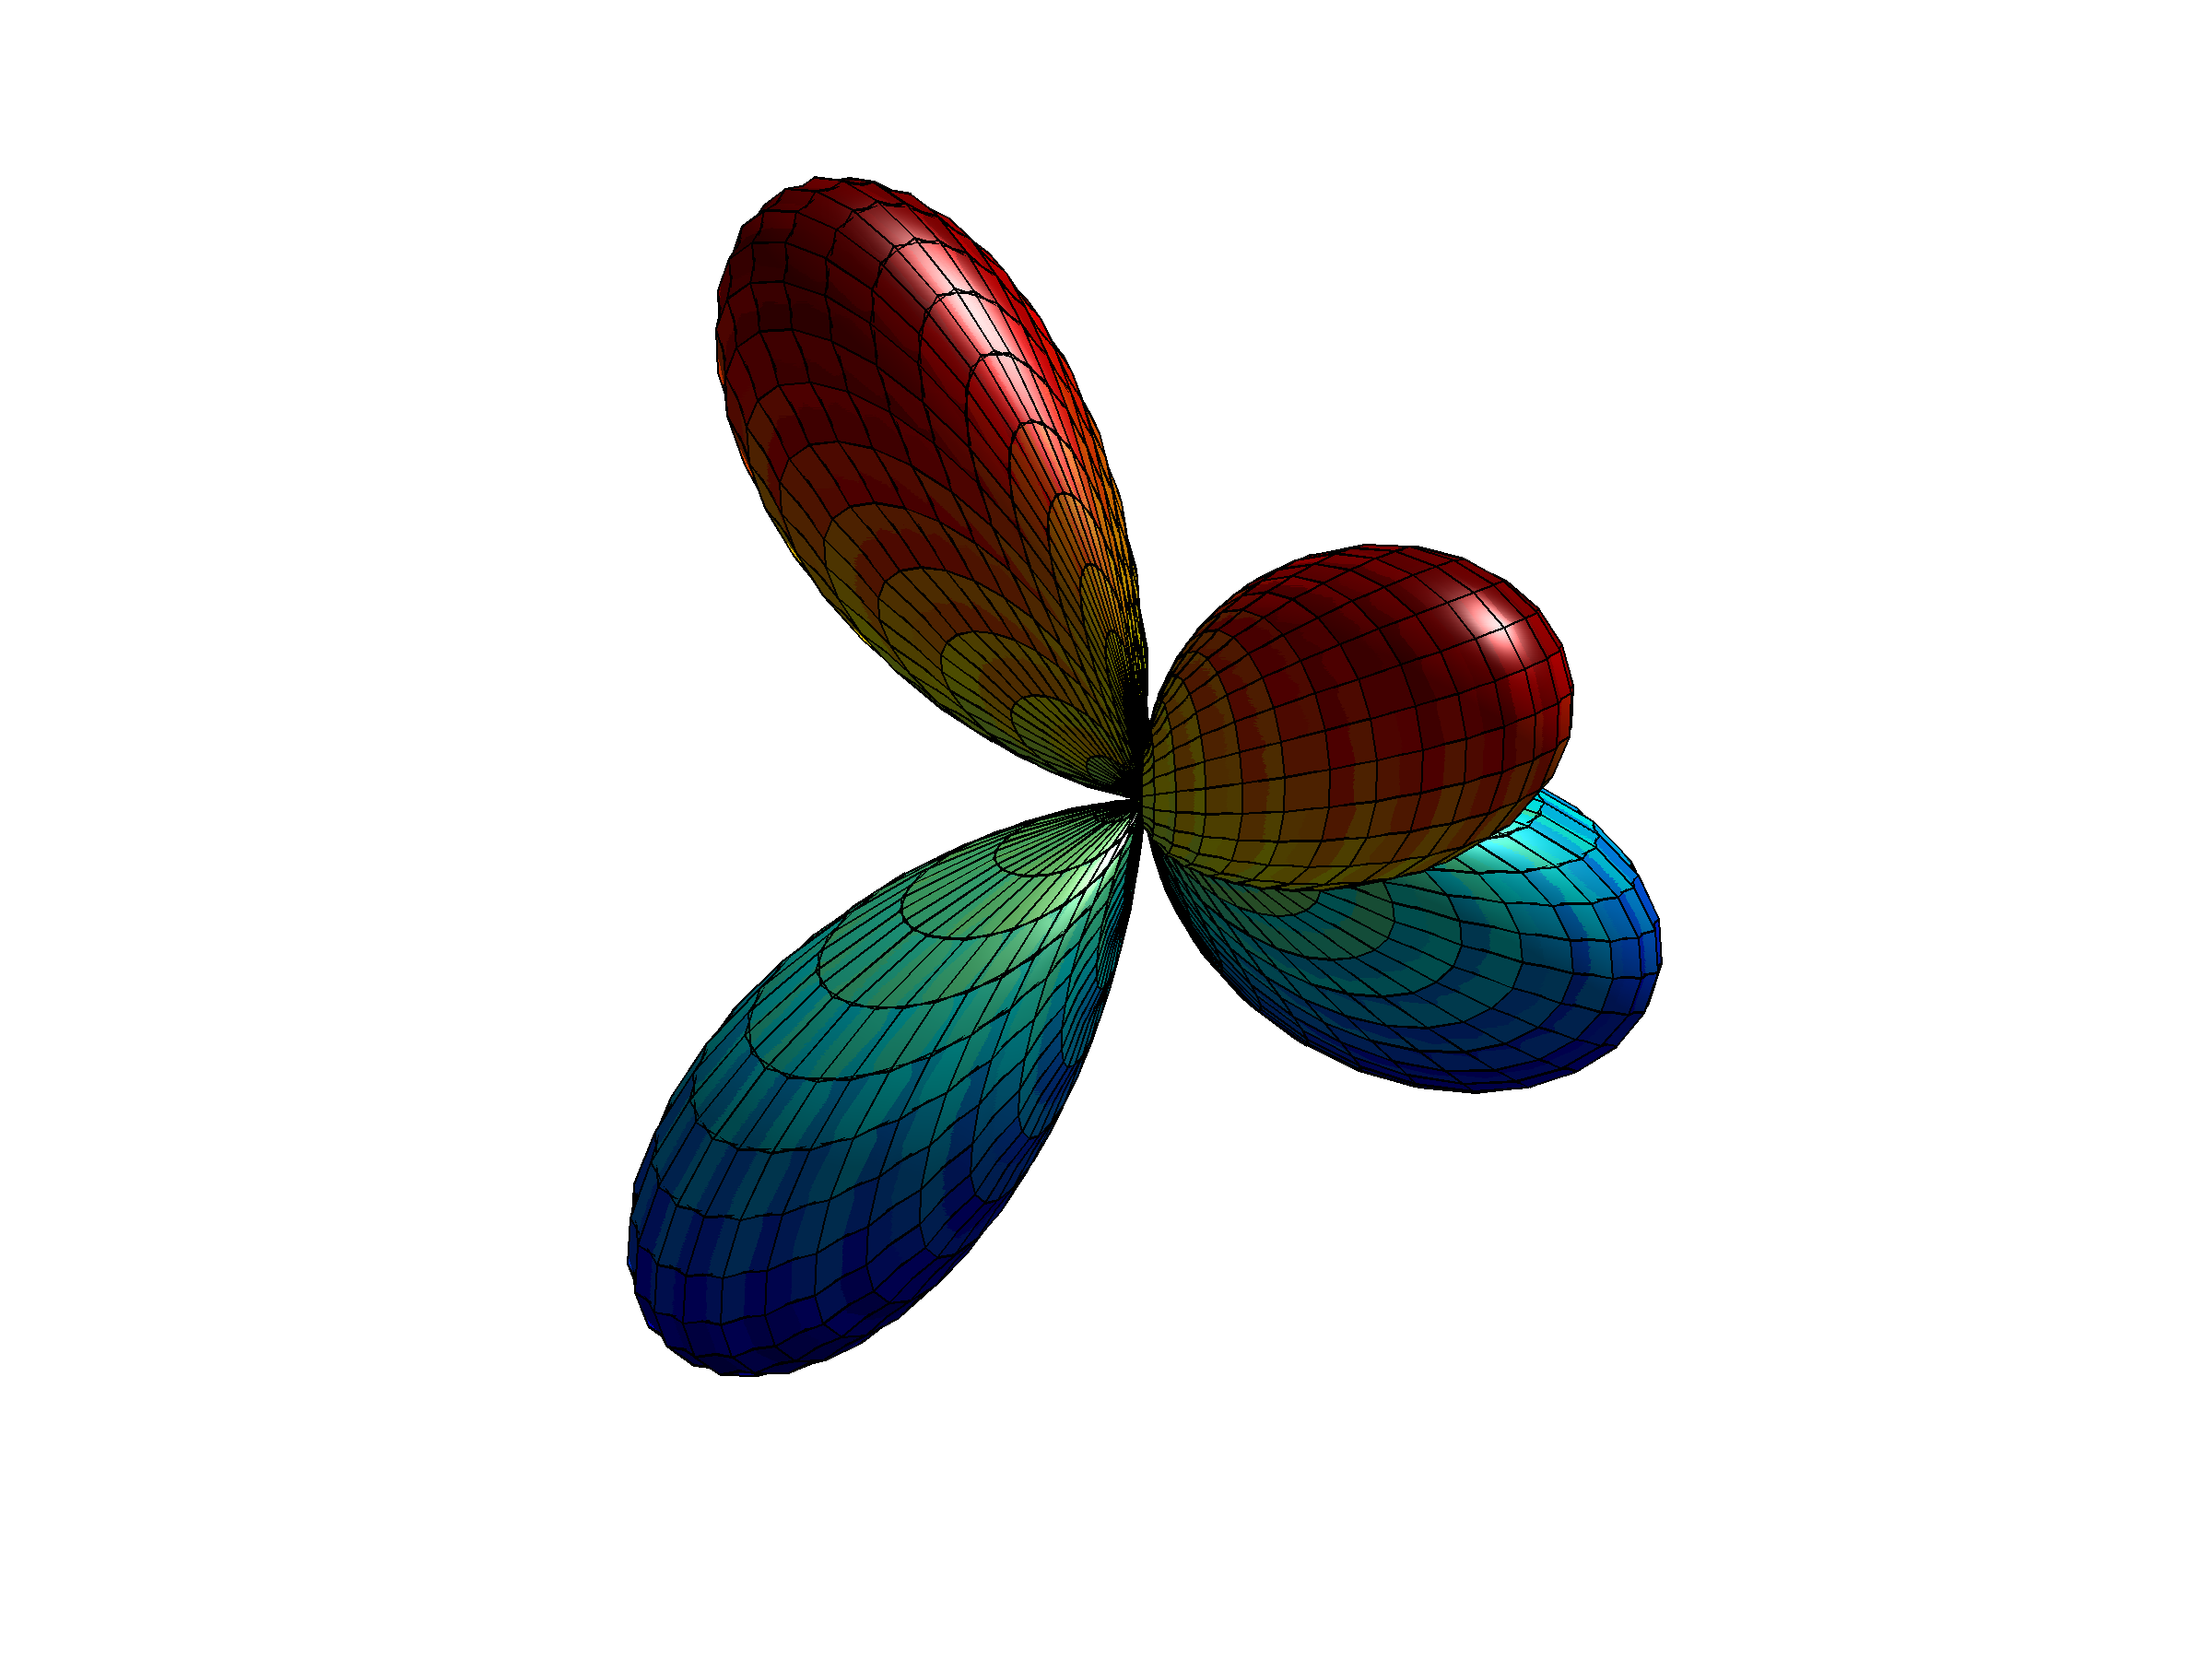
\includegraphics[width=\textwidth]{figures/appendices/Y_3_2.png}
		\caption{}
	\end{subfigure}
	\vfill
	\begin{subfigure}[b]{0.40\textwidth}
		\centering
		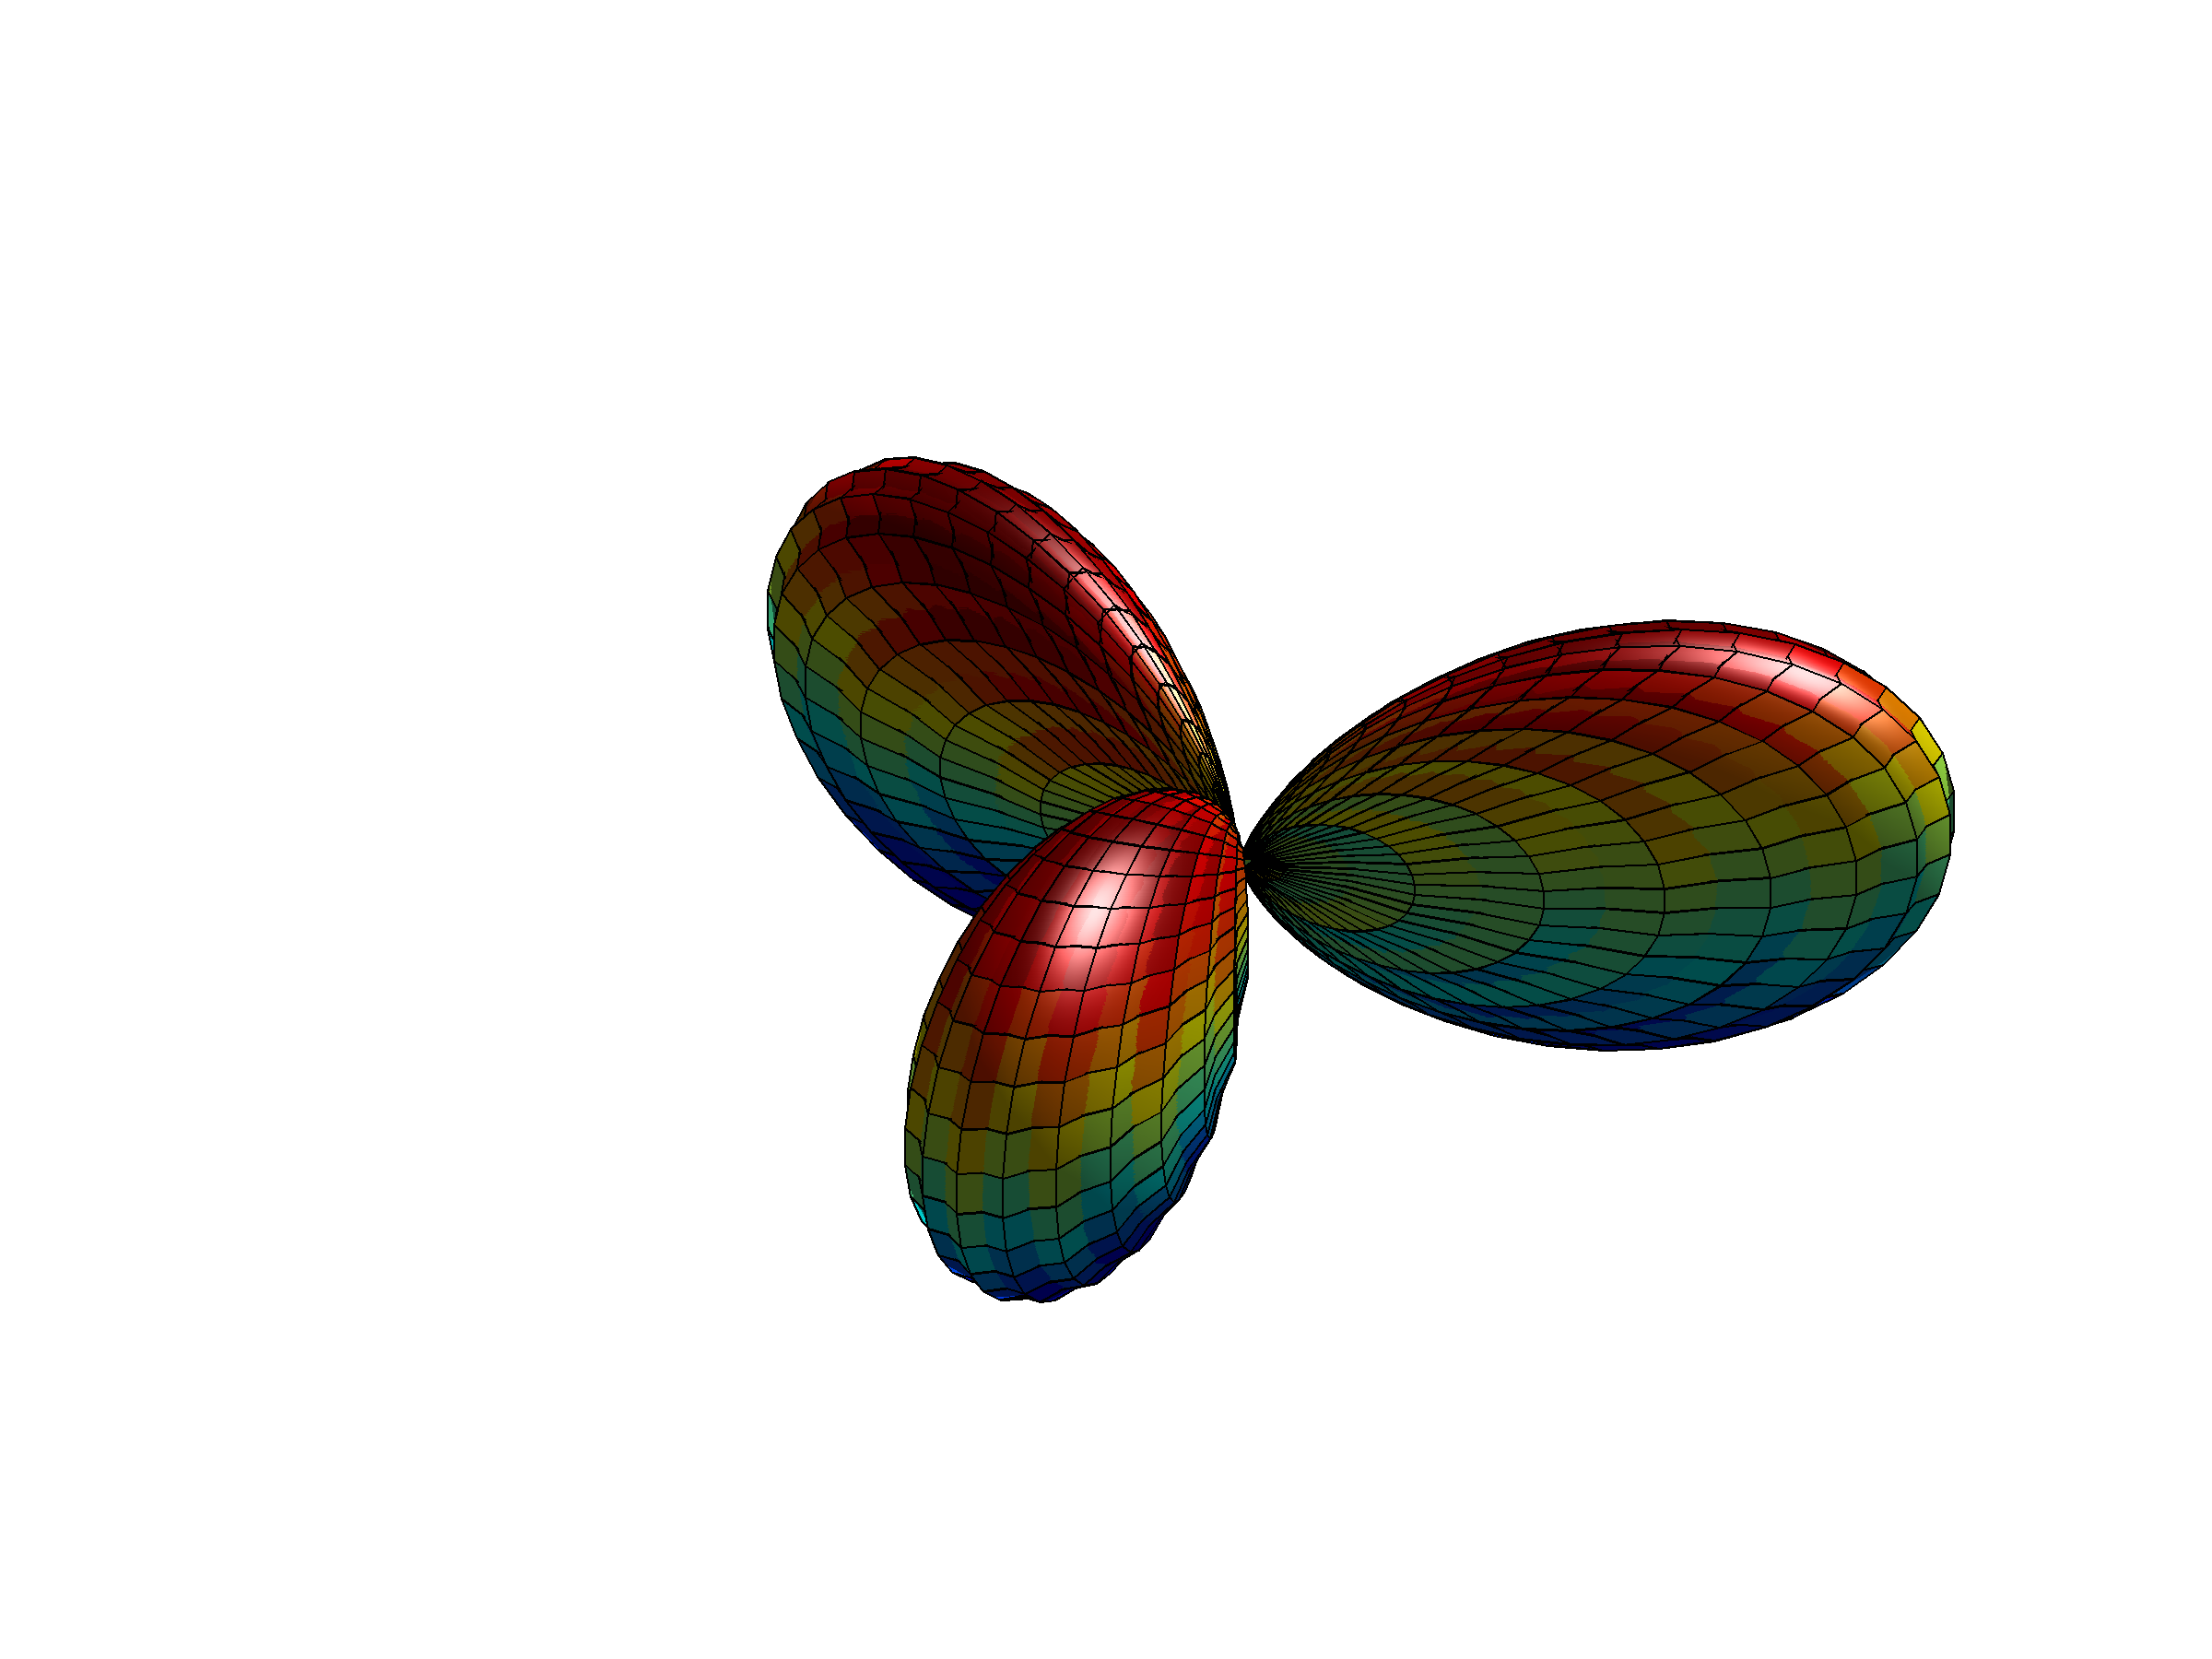
\includegraphics[width=\textwidth]{figures/appendices/Y_3_-3.png}
		\caption{}
	\end{subfigure}
	\hfill
	\begin{subfigure}[b]{0.40\textwidth}
		\centering
		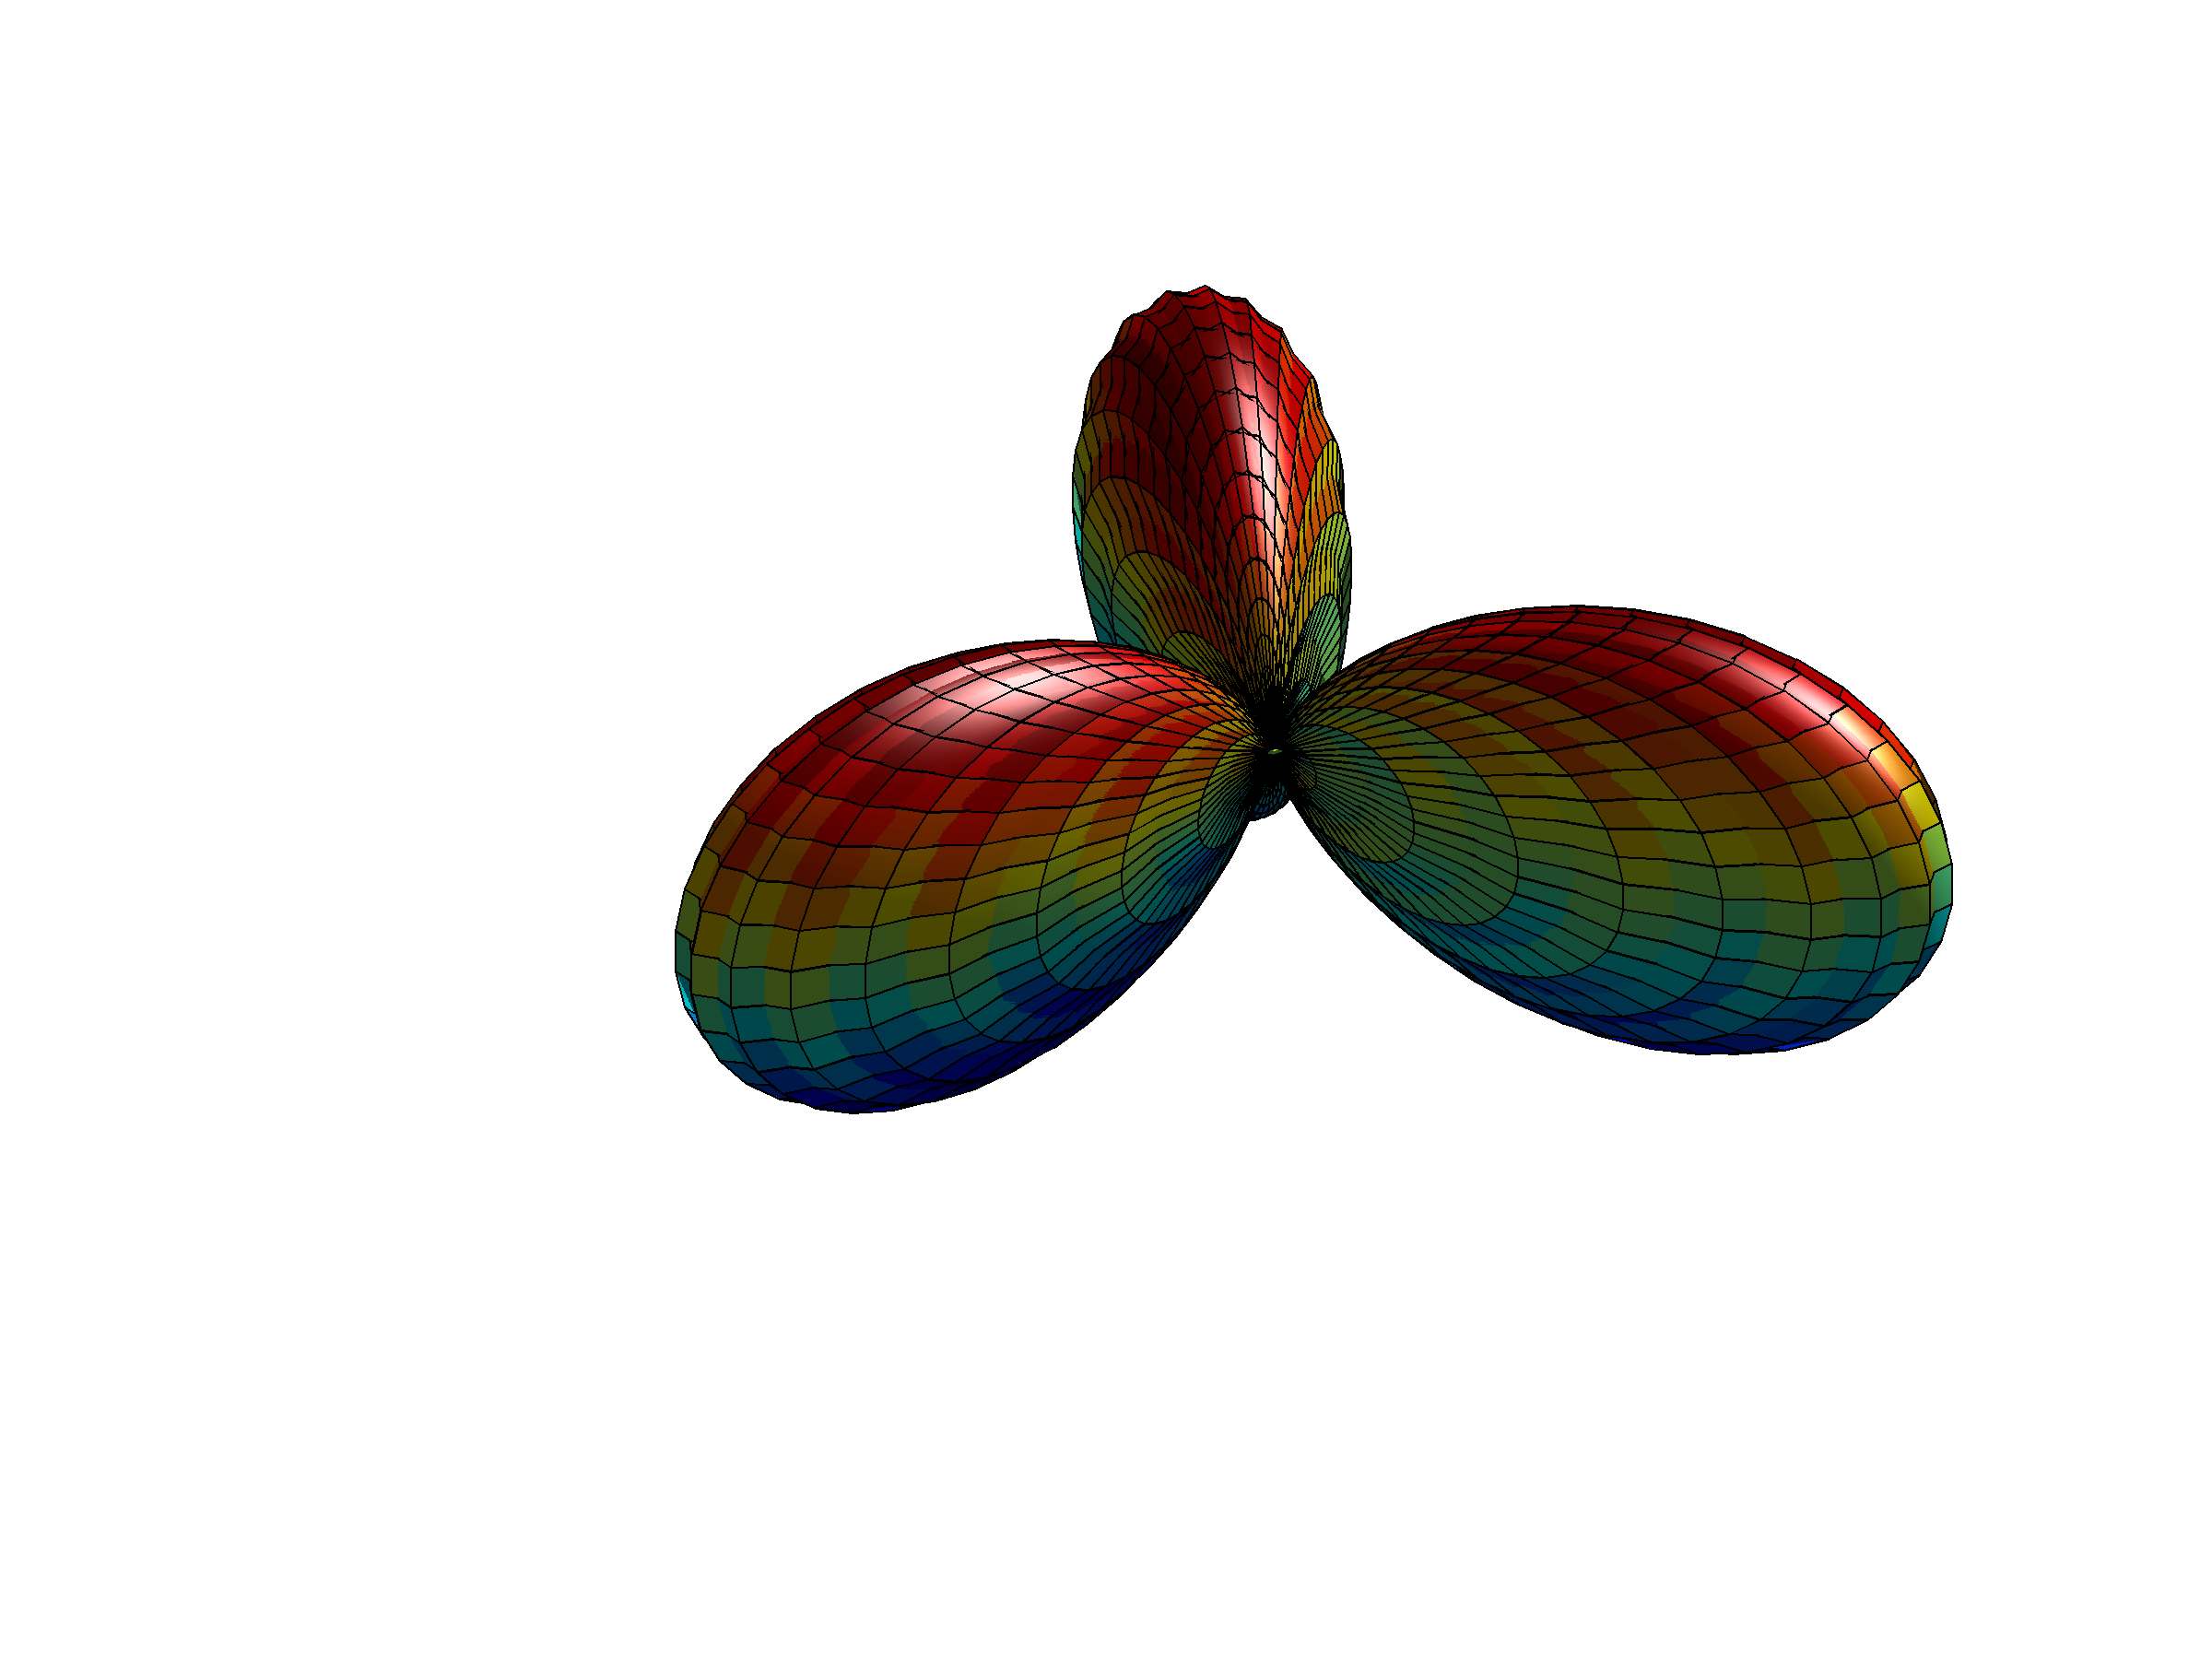
\includegraphics[width=\textwidth]{figures/appendices/Y_3_3.png}
		\caption{}
	\end{subfigure}
\caption{Spherical harmonic functions of degree 3: (a) $Y_{3}^{0}$, (b) $Y_{3}^{-1}$, (c) $Y_{3}^{1}$, (d) $Y_{3}^{-2}$, (e) $Y_{3}^{2}$, (f) $Y_{3}^{-3}$, and (g) $Y_{3}^{3}$.}
\end{figure}

